\documentclass[pdftex,11pt,a4paper,twoside]{report}

\usepackage{sty/pdf_course_profile}

%\title{Cours d'�lectricit�}

\title{\begin{flushright}
    \rule{17cm}{1mm}\\
    \vspace{8mm}
    \huge{\bf{Traitement du signal}}\\
	\vspace{4mm}
    \rule{17cm}{1mm}\\
    \large{Cours du CNAM - CPDA - 2012}\\
    \large{modifi� le }\today\\
    \large{Version 0.5.1}
    \end{flushright}
}

\author{\begin{flushright}
	\textbf{Guillaume Pellerin$^1$}\\
	\end{flushright}
    \vspace{12cm}
	\begin{center}
    \small{
    $^1$ Laboratoire d'Acoustique, Conservatoire National des Arts et M�tiers\\
    <\href{mailto:guillaume.pellerin@parisson.com}{guillaume.pellerin@parisson.com}>\\
     \vspace{0.5cm}
    }
    \end{center}}

\begin{document}

\maketitle

\newpage
Ce cours enseign� au Conservatoire National des Arts et M�tiers (CNAM) de Paris est destin� � introduire les notions th�oriques et pratiques du traitement du signal � un niveau Bac +2 ou +3.

Trois parties se distinguent pour s�parer tout d'abord les �l�ments th�oriques qui fondent la \textbf{th�orie du traitement de signal} par les m�thodes de Fourier, puis une synth�se des diff�rents \textbf{modes de repr�sentation des signaux} notamment celui du spectrogramme, et enfin une introduction � la \textbf{th�orie du filtrage num�rique}.\newline
%
% Comme vous le verrez, cette premi�re version tente un parcours non-exhaustif des fondements de l'acoustique architecturale. La plupart des �l�ments de ce polycopi� ont �t� tir�s des cours personnels de \textbf{Manuel Melon} (Ma�tre de Conf�rences au CNAM) \cite{melon} pour les deux premiers chap�tres, de \textbf{Jean-Dominique Polack} (Professeur des Universit�s et Directeur du Laboratoire d'Acoustique Musicale de Paris VI) \cite{polack_salles} pour les deux chapitres suivants et du livre de \textbf{Jacques Jouhaneau} (Professeur titulaire de la Chaire d'Acoustique du CNAM) \cite{jouhaneau} pour de tr�s nombreuses r�f�rences. Je les remercie tous sinc�rement de leur aide.\newline

Ce document est en constante �volution. Certaines parties seront revues ou corrig�es dans les versions ult�rieures. Les mises � jour seront disponibles sur l'adresse web indiqu�e en page de garde et je vous invite donc � la consulter r�guli�rement.

Il est publi� selon les termes de la licence Creative Commons by-nc-sa 2.0 France :

\url{http://creativecommons.org/licenses/by-nc-sa/2.0/fr/}

\begin{figure}[b]
  
\includegraphics[width=4cm]{img/Logo_cnam_new.jpg}
  \large{Copyright (C) 2006-2011 Guillaume Pellerin}
\end{figure}


\tableofcontents
\cleardoublepage
\renewcommand{\labelitemi}{$\bullet$}

\chapter{Les signaux}
\section{Pr�ambule}

L'information, qui se pr�sente � nous lors de l'observation d'un ph�nom�ne, se manifeste sous forme d'une ou plusieurs grandeurs physiques qui se d�roulent � la fois dans le temps et dans l'espace. Dans les probl�mes rencontr�s en pratique, on est souvent amen� � s'int�resser plus particuli�rement � l'un ou l'autre de ces deux aspects. On d�signe alors par le terme de \textbf{signal} l'�volution temporelle, tandis que l'on d�signe par le terme d'\textbf{image} l'�volution spatiale.

Les diff�rentes op�rations que l'on fait subir aux signaux n�cessitent des outils math�matiques appropri�s qui sont � la base du traitement du signal. Dans ce cours nous envisageons l'�tude de certains de ces outils. La th�orie du signal propose de mod�liser la grandeur physique observ�e par un objet math�matique d�pendant de la variable r�elle $t$ repr�sentant le temps. Dans la suite, le  signal d�signera indiff�remment la grandeur physique observ�e ou l'objet math�matique servant � la mod�liser. Le figure \ref{ex_sig} donne un aper�u de la repr�sentation temporelle de la forme d'onde d'un signal musical.

\begin{figure}[h]
    \centering
    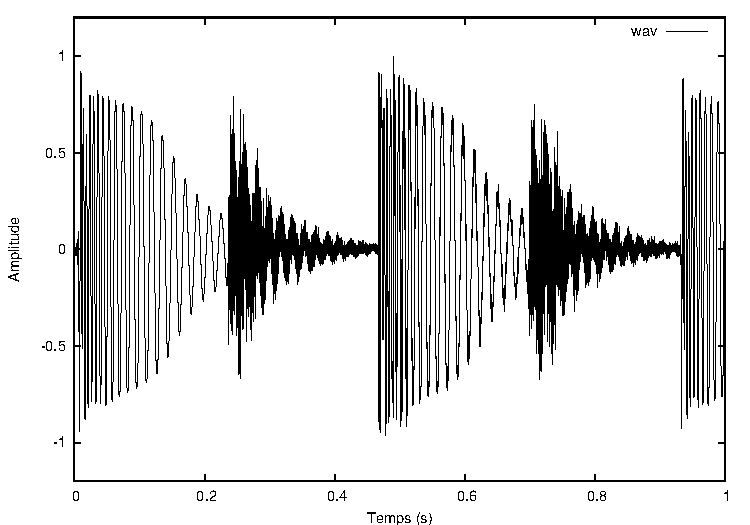
\includegraphics[width=12cm]{img/ex_sig}
    \caption{Exemple d'une r�pr�sentation temporelle d'un signal musical combinant un son de grosse caisse et celui d'une caisse claire.}
    \label{ex_sig}
\end{figure}


\section{Classification des signaux}

En th�orie du signal, on a l'habitude d'envisager plusieurs types de signaux. Pour rendre la suite de ce cours plus compr�hensible, nous pr�sentons dans cette section les diff�rents modes de classification des signaux.

\subsection{Classification dimensionnelle}

On peut diff�rentier les signaux selon leur nombre de variables libres. Par exemple un signal �lectrique $V(t)$ est un signal unidimensionnel d�pendant du temps. Une image statique en noir et blanc peut �tre mod�lis�e par un signal bidimensionnel correspondant � la brillance en fonction de la largeur et de la hauteur de l'image. Enfin, un film en noir et blanc peut �tre consid�r� comme une image fonction du temps, autrement dit mod�lis� par un signal tridimensionnel d�pendant de l'abscisse et de l'ordonn�e de l'image mais �galement du temps.

\subsection{Classification ph�nom�nologique}

La premi�re distinction porte sur notre capacit� � pr�dire l'�volution temporelle de la grandeur observ�e. Dans le cas d'un oscillateur sinuso�dal d'amplitude $A$ et de fr�quence $f_0$ par exemple, moyennant la mesure de $A$ et de $f_0$, on peut pr�dire la valeur de l'amplitude, � tout instant, par l'expression $x(t) = A\cos(2 \pi f_0 t)$. Un tel mod�le de signal est dit \textbf{d�terministe}. Il existe cependant des situations o� il n'est pas concevable d'expliciter, de cette fa�on, la forme de l'�volution temporelle du signal. C'est le cas, par exemple, pour la tension engendr�e � la sortie d'un microphone ou encore pour le courant �lectrique produit par l'agitation thermique des particules dans un conducteur (bruit de fond). On ne peut pas dire avec certitude combien vaudra $x(t)$ � l'instant $t$, mais on pourra �ventuellement supposer que cette grandeur est distribu�e suivant une certaine loi de probabilit�. On dit alors que le signal est \textbf{al�atoire}.

Pour simplifier, on peut dire que les signaux d�terministes sont des cas relativement th�oriques et id�aux, ou bien mod�lisent des signaux observ�s exp�rimentalement. Car en fait, tout signal physique r�el comporte une composante al�atoire correspondant � la perturbation externe.

\subsection{Classification morphologique}

Si, comme c'est le cas pour le signal $x(t) = Acos(2\pi f_0 t)$, o� $t\in\mathbb{R}$ et $A\in\mathbb{R}$, on dit que le signal est � temps continu. Toutefois on rencontre aussi en traitement du signal des grandeurs qui �voluent uniquement � des instants discrets $t_n$ o� $n$ est un entier. On parle alors de signal � temps discret ou encore de signal num�rique. En terme math�matique, un signal � temps continu est une fonction du temps tandis qu'un signal � temps discret est une suite. Le d�veloppement et l'essor des techniques num�riques ont fait que les probl�mes portant sur le traitements des signaux � temps discret ont pris une place majeure aujourd'hui, compar�e � celle qu'occupent les traitements portant sur les signaux � temps continu. C'est pourquoi ce cours est centre avant tout sur les probl�mes de temps discret et sur le passage du temps continu au temps discret (principe de l'�chantillonnage).

Il est �galement possible de discr�tiser le signal en amplitude. On appelle cela la \textbf{quantification} du signal.

\newpage
\subsection{Classification �nerg�tique}

On distingue en particulier deux types de signaux�:

\begin{itemize}
\item les signaux � �nergie finie comme tous les signaux physiques,
\item les signaux � puissance moyenne finie comme par exemple un signal sinuso�dal.
\end{itemize}


\section{Signaux et distributions classiques}

\subsection{Fen�tre rectangulaire ou Porte}

Soit $t \in \mathbb{R}$. Un signal rectangulaire s'�crit :

\begin{equation}
\boxed{\Pi_{2a}(t)}
\end{equation}

La repr�sentation graphique d'un signal porte est donn�e � la figure \ref{sig_porte}.

\begin{figure}[h]
    \centering
    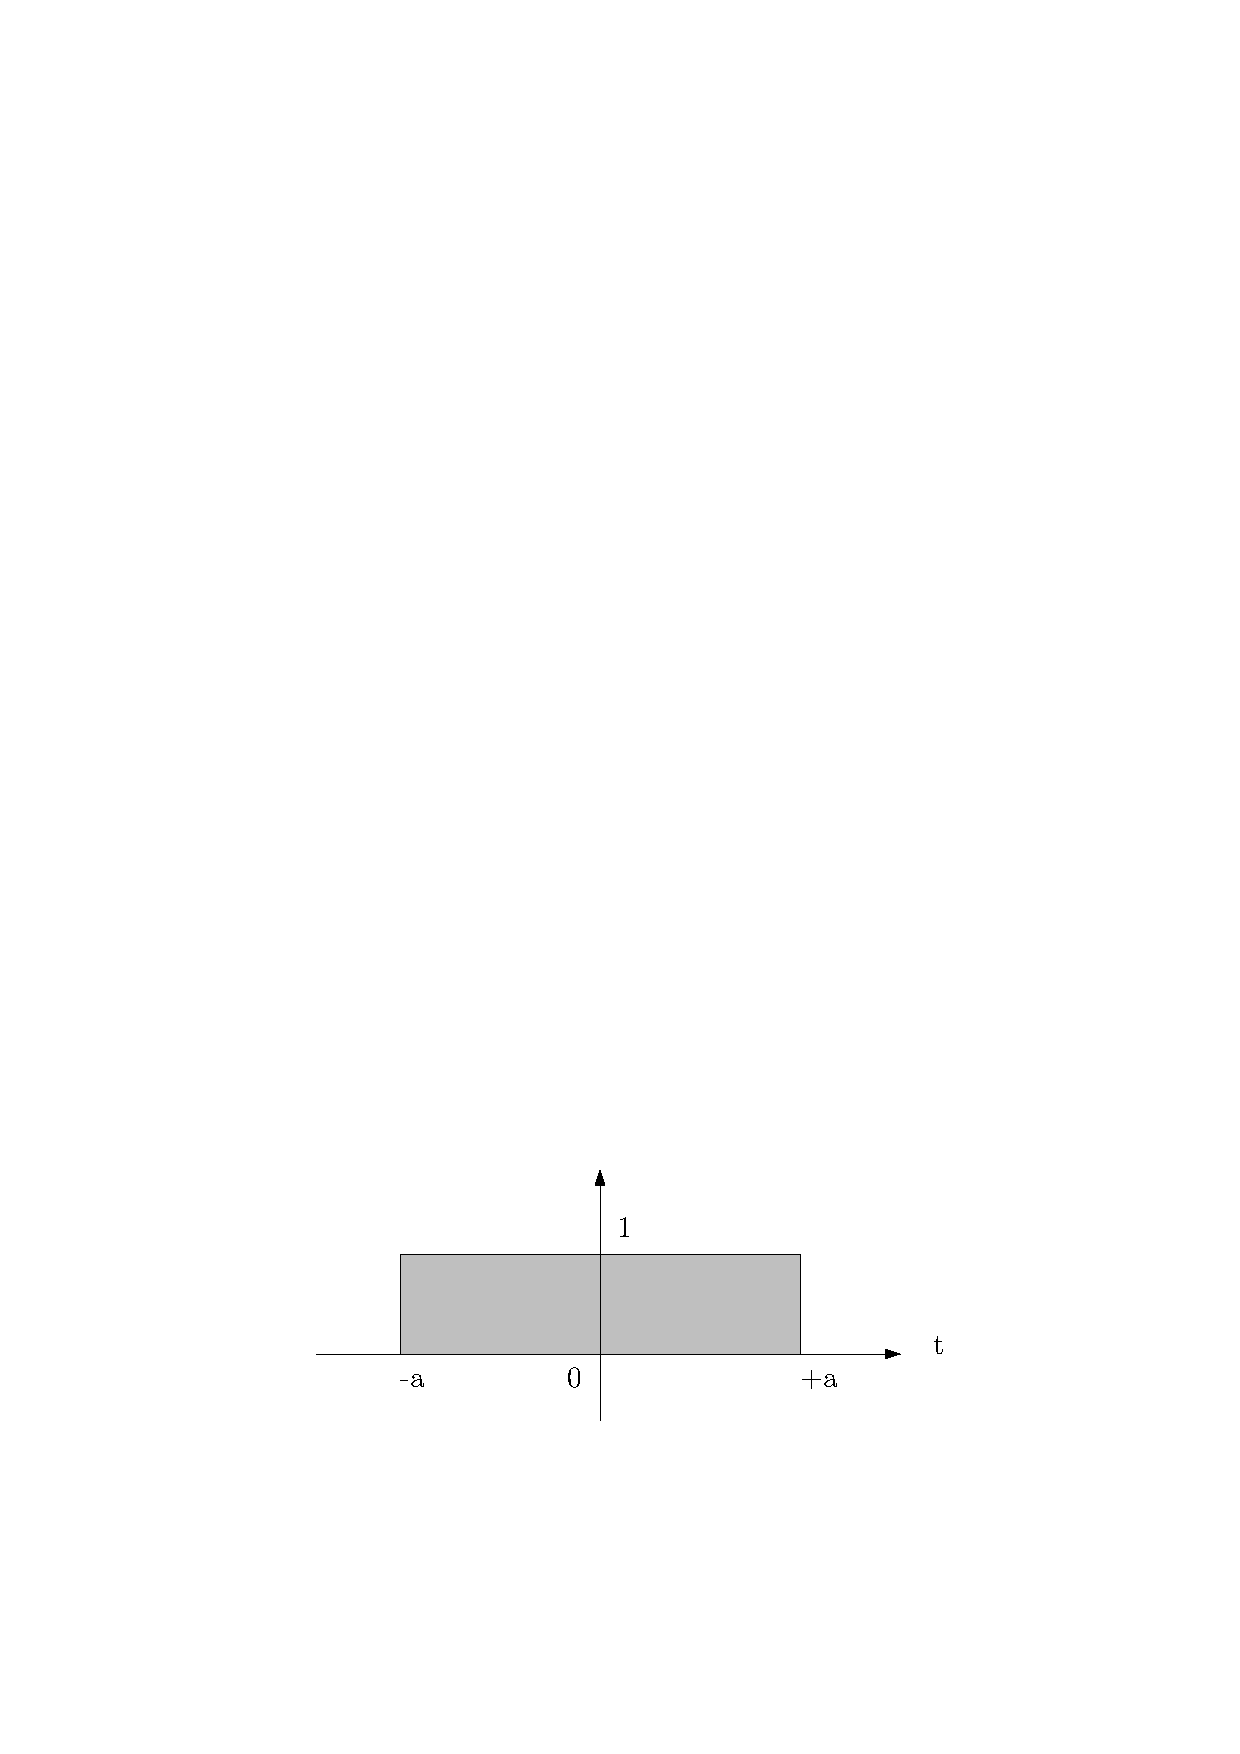
\includegraphics[width=8cm]{img/sig_porte}
    \caption{R�pr�sentation temporelle d'un signal rectangulaire ou << porte >>.}
    \label{sig_porte}
\end{figure}


\subsection{Impulsion de Dirac}

Les propri�t�s de l'impulsion de Dirac sont identiques � celles d'un signal rectangulaire dont la largeur tend vers 0 et la hauteur vers l'infini, � surface constante. Soit $t \in \mathbb{R}$ et $t_0 \in \mathbb{R}$. L'impulsion situ�e au temps $t_0$ s'�crit :

\begin{equation}
\boxed{\delta(t-t_0)}
\end{equation}

Il est souvent utilis� pour d�terminer la r�ponse impulsionnelle d'un syst�me dynamique. Une repr�sentation est donn�e � la figure \ref{sig_dirac}.

\begin{figure}[h]
    \centering
    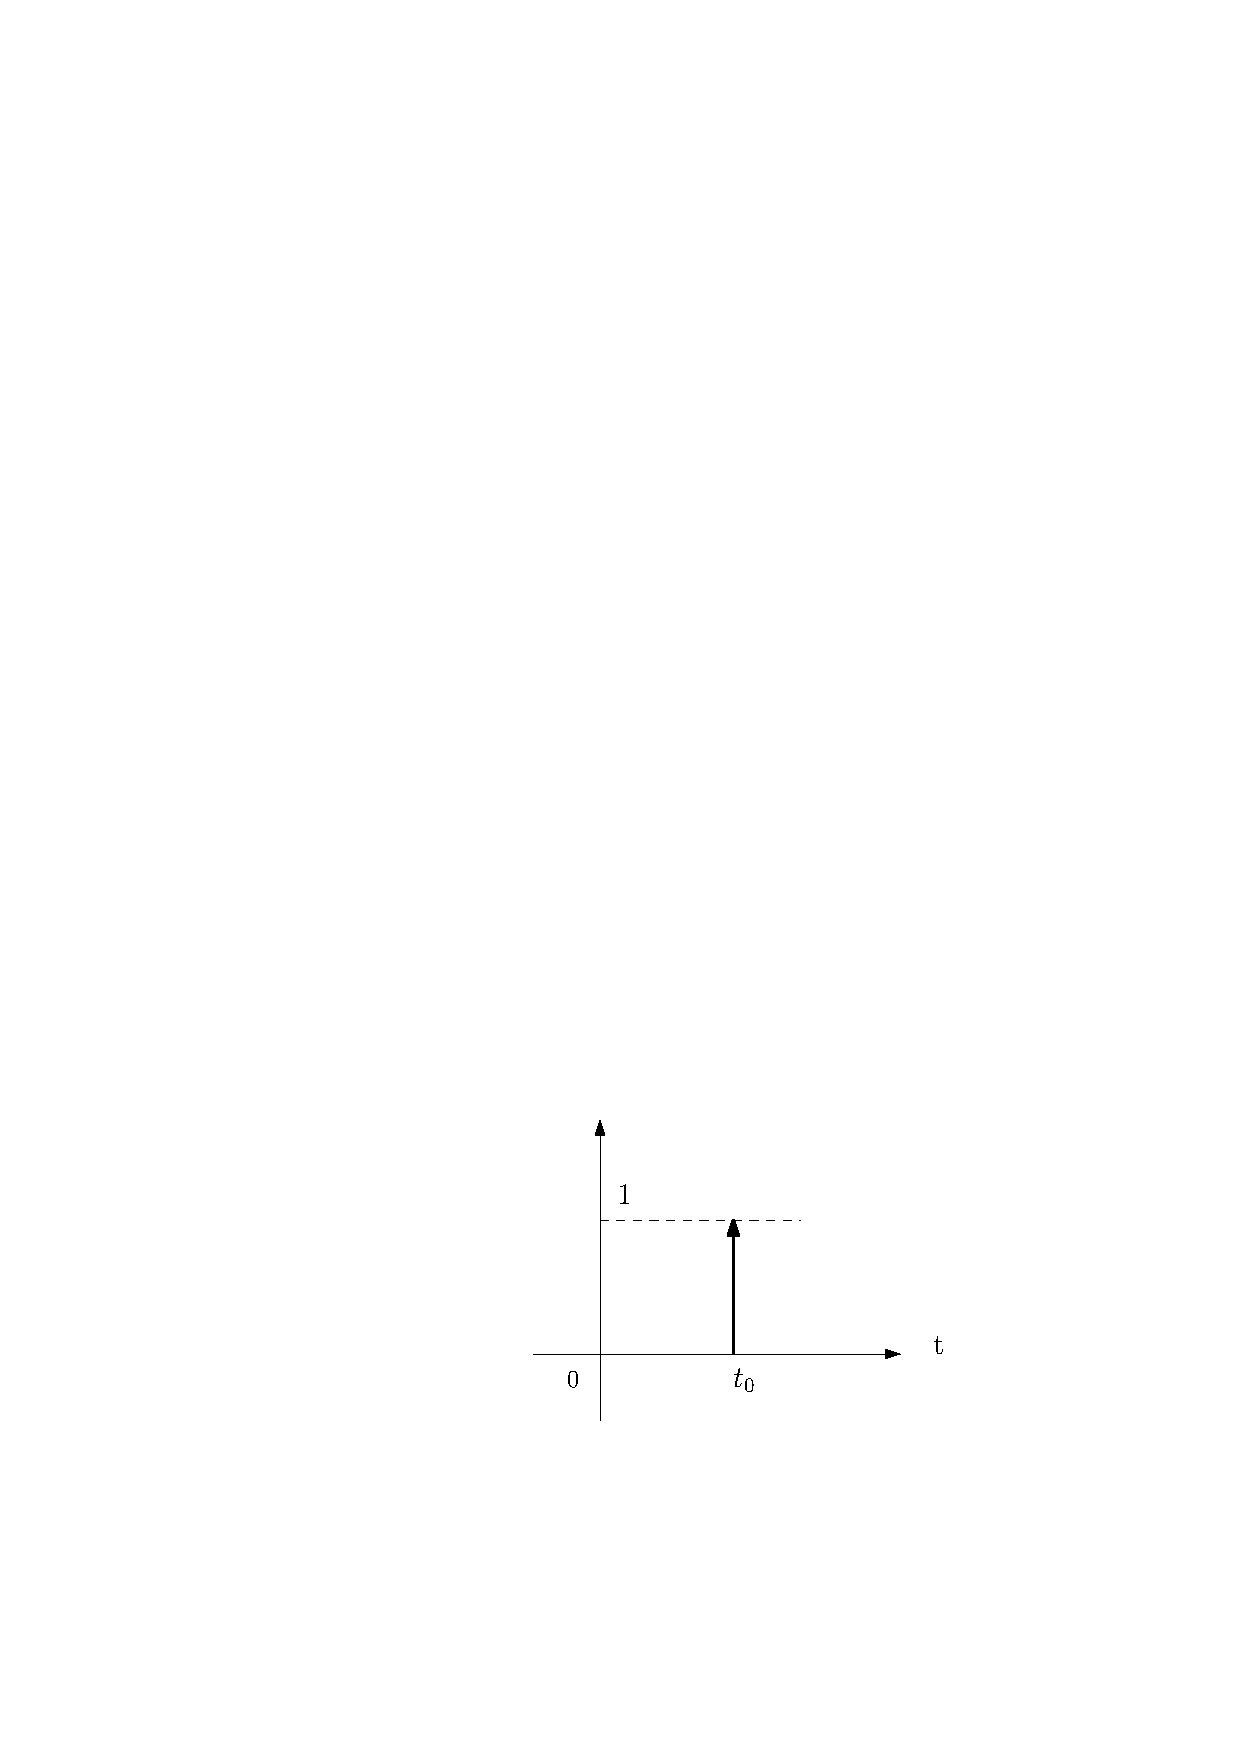
\includegraphics[width=6cm]{img/sig_dirac}
    \caption{R�pr�sentation temporelle d'une impulsion de Dirac.}
    \label{sig_dirac}
\end{figure}

\subsection{<<�Peigne�>> de Dirac}
Soit $T$ une p�riode en secondes, $t\in\mathbb{R}$, et $i\in\mathbb{N}$ et $n\in\mathbb{N}$. Le peigne de Dirac correspond � une p�riodisation d'impulsions de Dirac tous les $iT$ sur tout l'axe temporel (aussi bien $t<0$  que $t> 0$). Il s'�crit :

\begin{equation}
\boxed{\Psi_T(t) = \sum_{i=-\infty}^{+\infty} \delta (t-iT)}
\end{equation}

Une repr�sentation dun peigne de Dirac est donn�e � la figure \ref{sig_peigne}.

\begin{figure}[h]
    \centering
    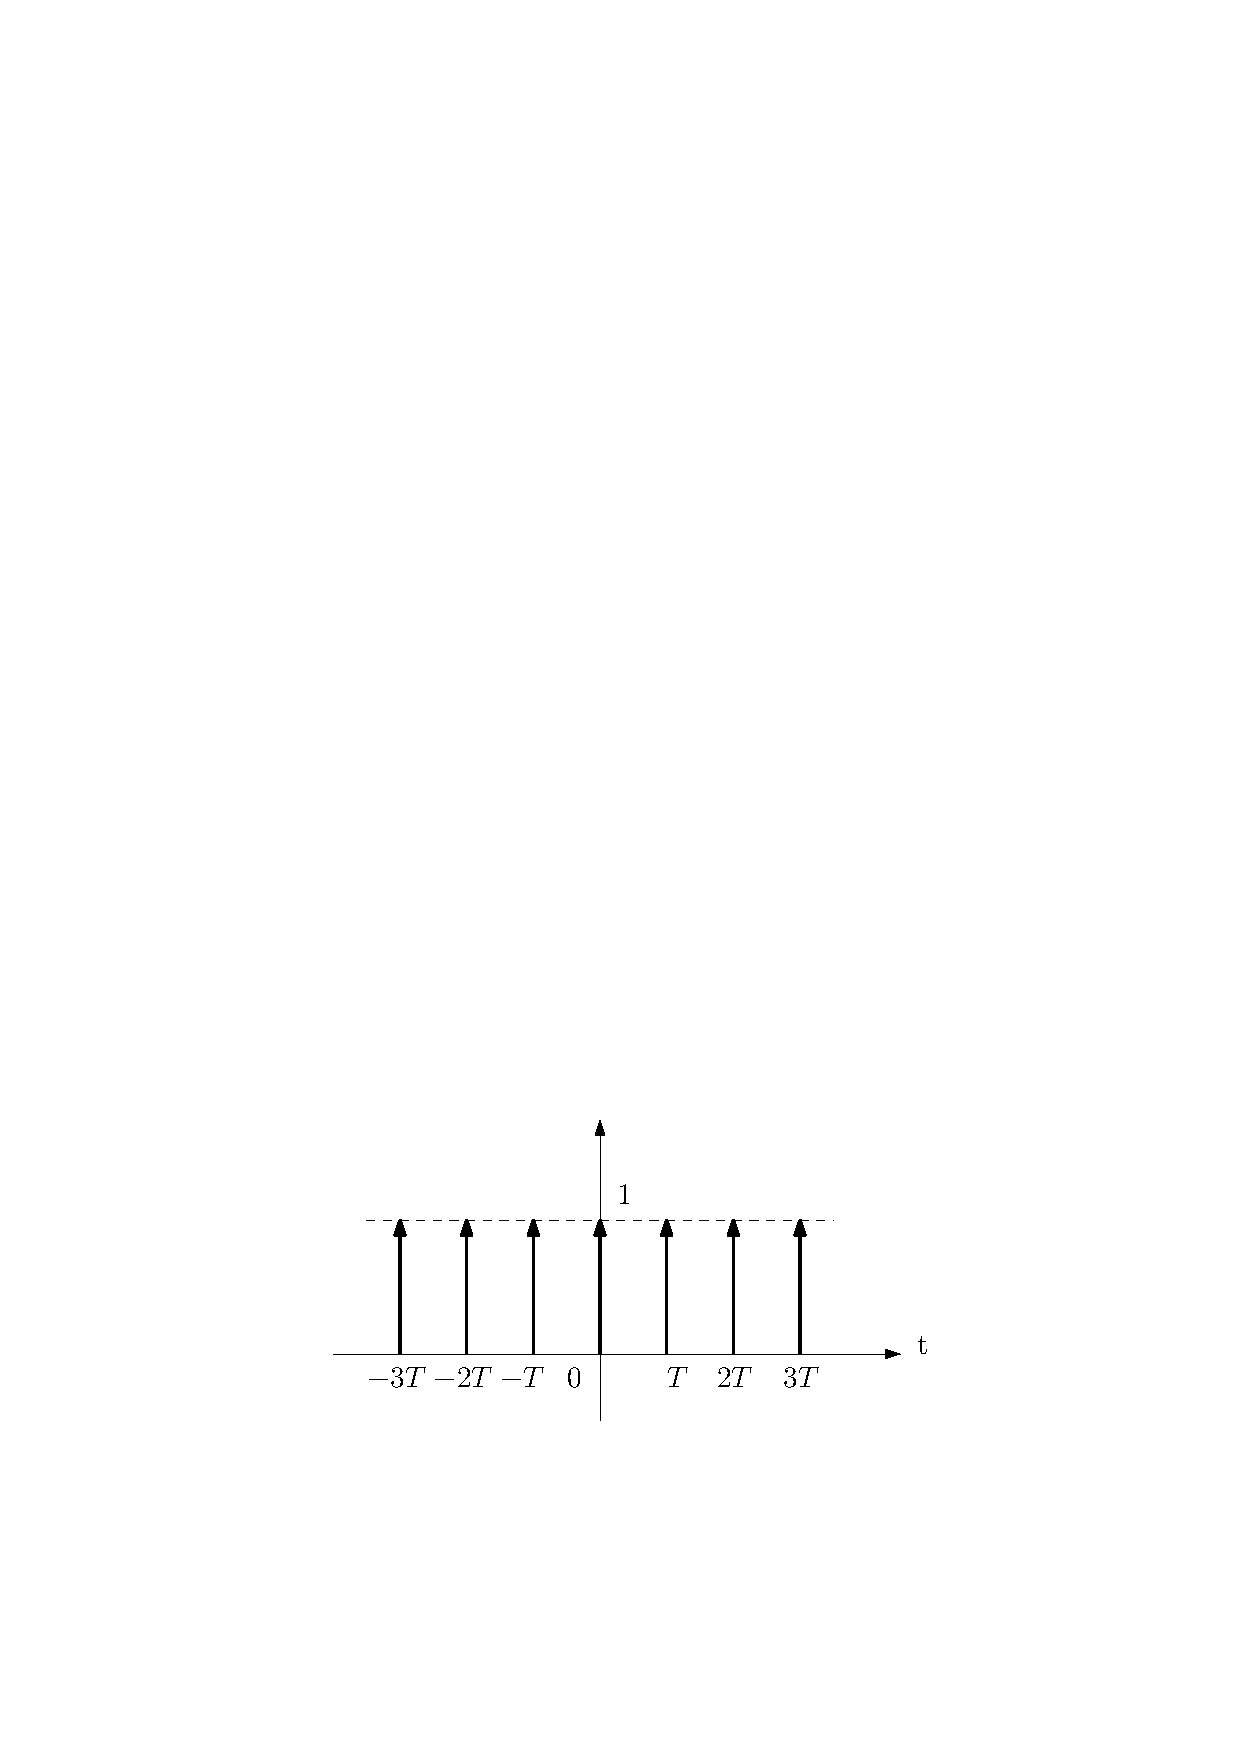
\includegraphics[width=8cm]{img/sig_train_dirac}
    \caption{R�pr�sentation temporelle d'un peigne de Dirac.}
    \label{sig_peigne}
\end{figure}


\subsection{Sinus cardinal}

Soit $t \in \mathbb{R}\backslash \lbrace 0 \rbrace$. Le sinus cardinal se d�finit par la formule�:

\begin{equation}
\boxed{\mathrm{sinc} (t) = \frac{\sin(t)}{t}}
\end{equation}

Une repr�sentation est donn�e � la figure \ref{sin_card}.

\begin{figure}[h]
    \centering
    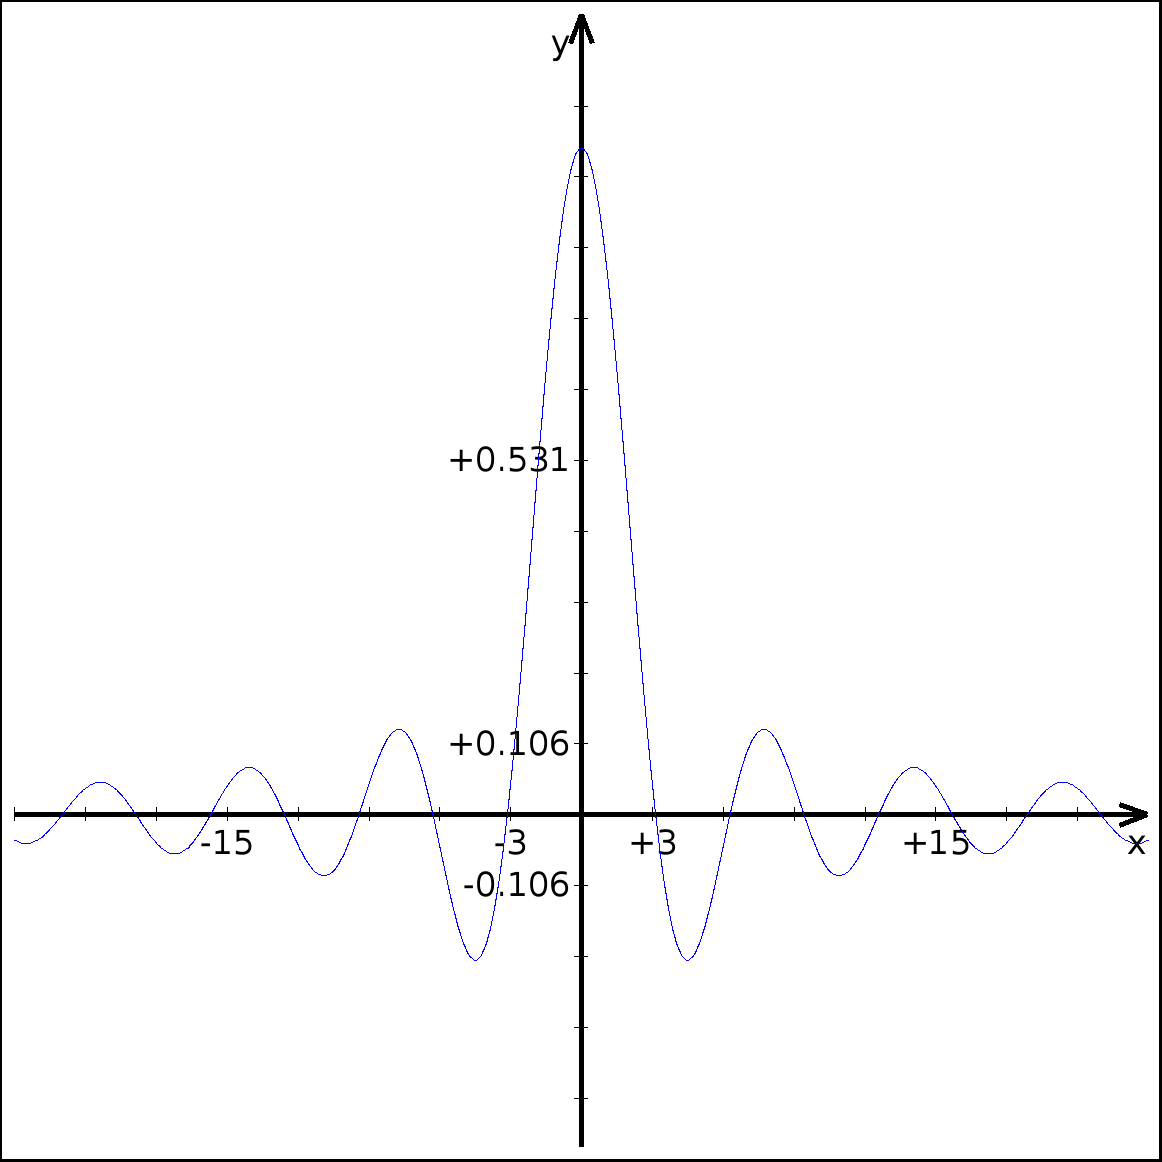
\includegraphics[width=10cm]{img/sinc}
    \caption{R�pr�sentation temporelle du sinus cardinal : $y=\frac{\sin(x)}{x}$ ($x\texttt{} \in \mathbb{R}\backslash \lbrace 0 \rbrace$).}
    \label{sin_card}
\end{figure}

\section{Evaluation de la similitude entre deux signaux}

Il existe en traitement du signal des outils math�matiques qui permettent d'�valuer la similitude entre deux signaux :

\begin{itemize}
\item au niveau de leur �volution temporelle gr�ce  � la fonction d'inter ou d'auto-corr�lation.
\item au niveau de leur composition spectrale gr�ce � la fonction de densit� spectrale.
\end{itemize}


\subsection{Les fonctions d'inter-corr�lation et d'auto-corr�lation}\label{intercorr}

La fonction d'\textbf{intercorr�lation} donne une quantit� li�e � la similitude entre deux signaux. Elle se d�finit par la formule suivante�:

\begin{equation}\label{inter_cor}
\varphi_{xy}(\tau)=\int_{-\infty}^{+\infty}x^*(t) y(t+\tau) \ud t
\end{equation}

o� $x^*(t)$ est le conjugu� de $x(t)$. Cette fonction renvoie un maximum lorsque les deux fonctions deviennent les plus similaires � t donn�e. La fonction d'\textbf{autocorr�lation} est un cas particulier de la fonction d'intercorr�lation pour laquelle $y(t) = x(t)$. Elle s'�crit donc�:

\begin{equation}\label{auto_cor}
\varphi_{x}(\tau)=\int_{-\infty}^{+\infty}x^*(t) x(t+\tau) \ud t
\end{equation}

La fonction d'autocorr�lation mesure ainsi la similitude de $x(t)$ avec une version d�call�e de $x(t)$. Elle atteint un maximum pour le temps $t_0$ auquel $x(t-t_0)$ ressemble le plus � $x(t)$.  C'est le cas particuli�rement pour les signaux p�riodiques qui reprennent la m�me valeur � chaque p�riode $T$. La fonction d'autocorr�lation permet ainsi d'estimer la p�riodicit� d'un signal semi-p�riodique en rep�rant le temps pour lequel elle atteint son maximum.

La fonction d'autocorr�lation permet �galement de calculer l'�nergie du signal puisque:

\begin{equation}\label{inter_cor2}
\varphi_{x}(0)=\int_{-\infty}^{+\infty} \vert x(t) \vert ^2 \ud t = E
\end{equation}





\chapter{Transform�es de signaux}
\section{Le produit de convolution}

On appelle produit de convolution \textbf{convolution} de $x(t)$ par $y(t)$ l'op�ration not�e $x(t) \star y(t)$ et d�finie par :

\begin{equation}\label{conv}
 \boxeq{x(t)\star y(t) = \int_{-\infty}^{+\infty}x(u)y(t-u)\ud u = \int_{-\infty}^{+\infty}x(t-u)y(u)\ud u}
\end{equation}

L'impulsion de Dirac est l'�l�ment neutre de la convolution. En effet :

\begin{equation}
x(t) \star \delta (t) = x(t)
\end{equation}

Lorsque l'on convolue un signal $x(t)$ � un Dirac situ� � un temps $t_0$, cela revient � retarder le signal $x(t)$ de $t_0$�:

\begin{equation}
x(t) \star \delta (t-t_0) = x(t-t_0)
\end{equation}

Par ailleurs, si l'on multiplie un signal $x(t)$ par un Dirac situ� � un temps $t_0$, cela revient � conna�tre la valeur que prend $x(t)$ en $t_0$ (comme si l'on relevait l'ordonn�e d'un point particulier d'une courbe)

\begin{equation}
x(t) \cdot \delta  (t-t_0) = x(t_0)
\end{equation}

De m�me, lorsque l'on convolue un signal $x(t)$ � un peigne de Dirac (de p�riode $T$), cela revient � <<�p�riodiser�>>  le signal $x(t)$ tous les $nT$�: on retarde le signal $x(t)$ de $T$, de $2T$, de $3T$, etc...

\begin{equation}
x(t) \star \Psi_T (t)  =  \Sigma x(t-nT)
\end{equation}

De fa�on plus g�n�rale, la convolution telle qu'elle est d�finie par sa formule math�matique, revient � retourner temporellement un des deux signaux (par exemple $x(t)$)  puis � le d�placer sur tout l'axe du temps  et � sommer toutes les multiplications de ce signal au deuxi�me signal $y(t)$.

Pour des exemples anim� de l'effet du produit de convolution (tr�s p�dagogique !), voir :�\\
\url{http://www.jhu.edu/~signals/convolve/index.html} \\
\url{http://www.jhu.edu/~signals/discreteconv2/index.html}

%Retournement temporel $t$ est un instant qui varie du signal $x$	dans le temps $u$ de  $-$  �  $+$.
%On fait ��glisser�� le signal $x(-u)$ selon l'axe du temps.
%On multiplie $y(u)$ par $x(t-u)$  pour chaque position de $t$ sur l'axe du temps et on somme tous les produits effectu�s.


\section{Rappels sur la d�composition en s�rie de Fourier des signaux p�riodiques}

Pour pouvoir analyser les signaux quelque soit leur nature, il est int�ressant de chercher des transformations qui mettent en �vidence les particularit�s de leur contenu temporel mais aussi fr�quentiel. Joseph Fourier a d�montr� que tout signal \textbf{p�riodique} peut �tre d�compos� en une somme de sinus et de cosinus �l�mentaires telle que :

\begin{equation}\label{DecompFour}
 \boxed{x(t)=a_0 + \sum_{n=1}^{+\infty}a_n\cos(2\pi n f_0 t)+\sum_{n=1}^{+\infty}b_n\sin(2\pi n f_0 t)}
\end{equation}

o� $f_0$ est appel�e la fr�quence \textbf{fondamentale}. Sauf effet particulier ou paradoxal, elle correspond � la hauteur principale per�ue d'un son. Les autres composantes sont des fr�quences sup�rieures � la fondamentale ($n>1$) et sont appel�es \textbf{harmoniques} du signal. Par exemple, dans le cas d'un son �mis par un instrument de musique, la fondamentale va correspondre � la note jou�e et les autres composantes vont correspondre � la <<�s�rie harmonique�>> de cette note (octave, puis quinte, puis octave, puis tierce, etc...). Cette s�rie correspond � des rapports de fr�quences (fondamental $f_0$, octave $= 2*f_0$, octave $+$ quinte $= 3*f_0$, etc...). Les harmoniques ne vont pas directement contribuer � la perception de la hauteur mais plut�t � la richesse du timbre du son. C'est par exemple la pr�sence d'harmoniques, entre autres, qui permet de diff�rentier une sinuso�de � $f_0$ d'une note de violon dont la fondamentale est � la m�me fr�quence.


\section{La transform�e de Fourier}

\subsection{D�finition de la transform�e de Fourier}

La transform�e de Fourier est une g�n�ralisation de la d�composition pr�cedente aux signaux non-p�riodiques. Soit $x(t)$ un signal quelconque, on note $X(f)$ ou $TF(x(t))$ sa transform�e de Fourier telle que�:

\begin{equation}\label{fourier}
 \boxeq{X(f)=TF(x(t))=\int_{-\infty}^{+\infty}x(t)e^{-i2\pi f t} \ud t}
\end{equation}

Inversement, on peut d�finir une transform�e de Fourier inverse $TF^{-1}$ telle que :

\begin{equation}\label{fourier_inv}
 \boxeq{x(t)=TF^{-1}(X(f))=\int_{-\infty}^{+\infty}X(f)e^{i2\pi f t} \ud f}
\end{equation}

$X(f)$ est une fonction complexe m�me si $x(t)$ est r�el. La transform�e de Fourier contient donc une partie r�elle et une partie imaginaire et est repr�sent�e facilement gr�ce � son \textbf{module} et � son \textbf{argument} : $\vert X(f) \vert$ est appel� \textbf{spectre d'amplitude} et $\mathrm{arg}(X(f))$ le \textbf{spectre de phase} du signal. La variable $f$ s'appelle la fr�quence dont l'unit� est le Hertz (en abr�g� : Hz).\\

\textbf{Remarques importantes:}
\begin{itemize}
 \item La repr�sentation compl�te d'une transform�e de Fourier n�cessite 2 graphiques : le module et la phase, ou bien la partie r�elle et le partie imaginaire.
 \item Pour repr�senter les transform�es de Fourier de signaux, il est commun�ment utilis� l'�chelle logarithmique. Pour un signal acoustique, par exemple, on calcule $20\log(\vert X(f) \vert / 2.10^{-5})$ et $\mathrm{arg}(X(f))$.\\
\end{itemize}

Ainsi, la transform�e de Fourier est un op�rateur math�matique qui permet d'analyser et de repr�senter un signal dans le domaine fr�quentiel. La $TF$ ne modifie pas le signal mais permet seulement de l'observer selon diff�rents points de vue (temporel ou fr�quentiel). Il est important de retenir que $x(t)$ et $X(f)$ sont deux descriptions �quivalentes du m�me signal. Ces deux fonctions contiennent la m�me information il s'agit juste de deux descriptions dans des domaines diff�rents.

$X(f)$ apporte des informations sur le syst�me physique � l'origine du signal. Elle permet par exemple de diff�rentier un son de trompette d'un son trombone, ou bien encore diff�rentes ondes c�r�brales, plus facilement qu'en observant le signal dans le domaine temporel. Le \textbf{contenu spectral} d'un signal est en effet assimilable � sa << carte d'identit� >>.


\subsection{Propri�t�s de la transform�e de Fourier}

\begin{itemize}
 \item \textbf{Lin�arit�}�:

\begin{equation}
 \boxeq{a x(t)+b y(t) \Leftrightarrow a X(f)+b Y(f)}
\end{equation}

\item \textbf{Produit de convolution}�:

\begin{equation}
 \boxeq{x(t).y(t) \Leftrightarrow   X(f) \star Y(f)}
\end{equation}

\begin{equation}
 \boxeq{x(t) \star y(t)  \Leftrightarrow  X(f) . Y(f)}
\end{equation}

Une multiplication dans un domaine correspond ainsi � un produit de convolution dans l'autre.\\

\item \textbf{Retard}�:

\begin{equation}
 \boxeq{x(t-t_0)   \Leftrightarrow  X(f) e^{-2i\pi f t_0}}
\end{equation}

\begin{equation}
 \boxeq{x(t) \cdot e^{2i\pi f_0 t} \Leftrightarrow  X(f-f_0)}
\end{equation}

Un retard temporel correspond ainsi � un d�phasage au niveau fr�quentiel, et inversement.\\

\item \textbf{Changement d'�chelle}�:

\begin{equation}
\boxeq{x(at) \Leftrightarrow \frac{1}{\vert a \vert} X \left(\frac{f}{a} \right)}
\end{equation}

\textbf{D�monstration.} Soient $x(t)$ et $y(t)$ deux fonctions temporelles avec $t \in \mathbb{R}$ telles que $y(t)=x(at)$ avec $a \in \mathbb{R}$. Leur transform�es de Fourier dans l'espace des fr�quences sont not�es respectivement $X(f)$ et $Y(f)$. On a alors :

\begin{eqnarray}
 Y(f) & = & \int_{-\infty}^{+\infty} y(t)e^{-2i\pi f t} \ud t\\
 & = & \int_{-\infty}^{+\infty} x(at)e^{-2i\pi f t} \ud t \label{dem_ft_ech}
\end{eqnarray}

Effectuons le changement de variable $u=at$, c'est-�-dire aussi $\ud u=a \ud t$, qui revient ici � un changement d'�chelle. L'�quation \ref{dem_ft_ech} devient :

\begin{eqnarray}
 Y(f) & = & \int_{-\infty}^{+\infty} x(u)e^{-\frac{2i\pi f u}{a}} \frac{\ud u}{a}\\
 & = & \frac{1}{\vert a \vert} \int_{-\infty}^{+\infty} x(u) e^{-2i\pi \frac{f}{a}u} \ud u\\
 & = & \frac{1}{\vert a \vert}X\left(\frac{f}{a}\right) \label{dem_ft_ech_2}
\end{eqnarray}

Cette loi montre que lorsqu'on diminue l'�chelle temporelle d'un signal ($a>1$), l'�chelle fr�quentielle augmente. Par exemple, si $x(t)$ est une sinuso�de de fr�quence $f_0$ telle que $x(t)=\sin(2\pi f_0 t)$, alors $X(f)=\delta(f-f_0)$, $y(t)=\sin(2\pi a f_0 t)$ et $Y(f)=\frac{1}{\vert a \vert}\delta(f-f_1)$ o� $f_1=a f_0$ (cf. figure \ref{sinus_ech}). Le facteur suppl�mentaire $\frac{1}{\vert a \vert}$ provient du principe de conservation d'�nergie appliqu� dans le domaine fr�quentiel.\\

\begin{figure}[tp]
    \centering
    \subfigure[Repr�sentation temporelle]{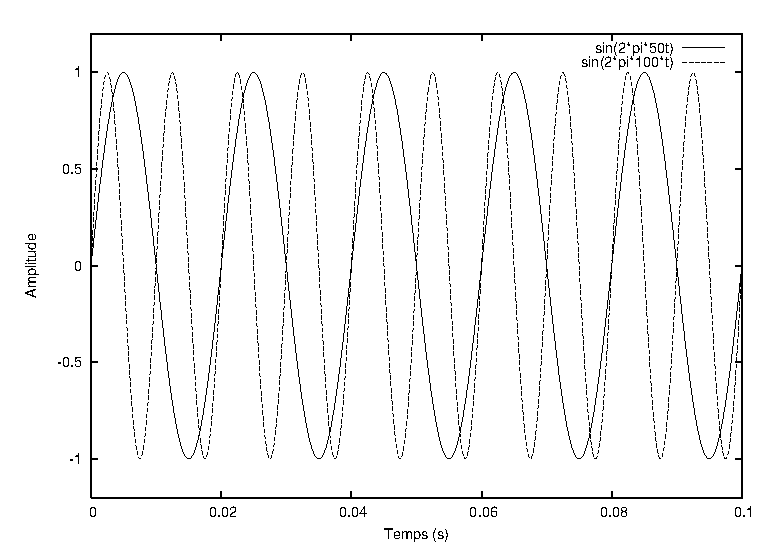
\includegraphics[width=8cm]{img/sinus_ech}}
    \subfigure[Repr�sentation fr�quentielle]{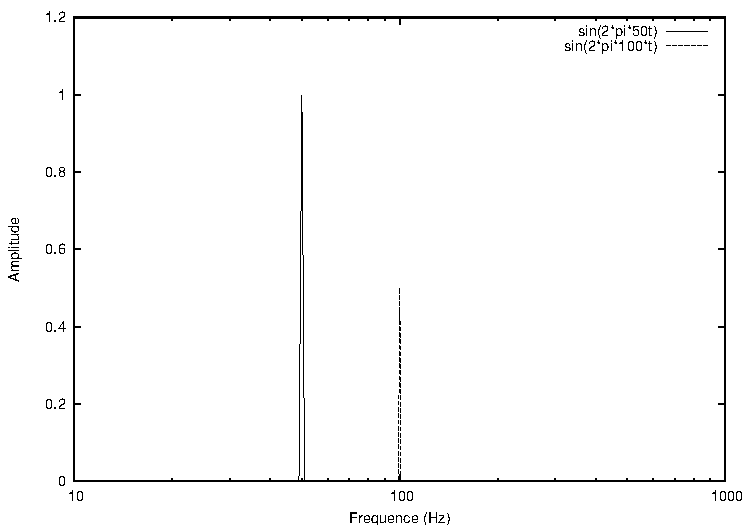
\includegraphics[width=8cm]{img/sinus_ech_ft}}
    \caption{Exemple d'application d'un facteur d'�chelle $a=2$ sur un signal sinuso�dal $x(t)$ de fr�quence $f_0=50\ \mathrm{Hz}$ tel que $x(t)=\sin(2\pi f_0 t)$.}
    \label{sinus_ech}
\end{figure}

\item \textbf{Th�or�me de Parseval}�:\\
Soit $E$ l'�nergie du signal. On peut d�montrer que :

\begin{equation}
 \boxeq{E = \int_{-\infty}^{+\infty} \vert x(t) \vert^2 \ud t   =   \int_{-\infty}^{+\infty}    \vert X(f) \vert^2 \ud f}
\end{equation}

\end{itemize}


\subsection{Les transform�es de Fourier de signaux courants}

\begin{itemize}
\item Dirac $\delta(t) \Leftrightarrow $ signal unit�
\item Signal porte  $\Leftrightarrow$ sinus cardinal
\item $\sin(2\pi f_0 t)  \Leftrightarrow  \frac{1}{2}[\delta(f-f_0)  + \delta(f+f_0)]$
\item la suite en cours...
\end{itemize}


\subsection{La fonction de densit� spectrale d'�nergie}

La fonction de densit� spectrale d'�nergie est la $TF$ de la fonction d'autocorr�lation vue au paragraphe \ref{intercorr}. Elle d�crit la r�partition de l'�nergie en fr�quence et on a :


\begin{equation}\label{PSD}
\Phi_{x}(f)= TF (\varphi_x(\tau))=\vert X(f) \vert ^2
\end{equation}


\section{L'�chantillonnage}\label{signum}

Les signaux num�riques d�rivent d�'un signal analogique par \textbf{�chantillonnage}. L'�chantillonnage est une op�ration qui consiste � pr�lever sur un signal � temps continu une suite de valeurs, prises en une suite d'instants $t_n$, $n\in \mathbb{Z}$. Dans la suite nous n'envisagerons que l'�chantillonnage est r�gulier, \cad que $t_n$ = $nT$.

Aujourd'hui l'int�r�t grandissant pour la conversion de signaux analogiques en signaux num�riques tient au fait qu'il devient de plus en plus simple d'appliquer des algorithmes d'analyse complexe avec l'aide des processeurs num�riques. En sciences physiques par exemple, il est fr�quent que les r�sultats exp�rimentaux soient sous forme d'une suite de valeurs num�riques. Les possibilit�s d'application du traitement num�rique des signaux sont d'autant plus nombreuses que la vitesse de calcul des microprocesseurs est �lev�e. Pour caract�riser et traiter un tel signal num�rique on peut utiliser les m�me concepts math�matiques que pour les signaux continus, � condition de les adapter aux contexte num�rique.


\subsection{D�finition de l'�chantillonnage}\label{sampling}

Le signal continu (analogique) peut �tre �chantillonn� (\cad discr�tis�) � une \textbf{fr�quence d'�chantillonnage} $f_e$ inverse de la \textbf{p�riode d'�chantillonnage} $T_e$ telle que $f_e= 1/T_e$. Cet �chantillonnage revient � multiplier le signal analogique par un peigne de Dirac de p�riode $T_e$.

Le signal �chantillonn� peut alors s'�crire�:

\begin{equation}
 x_e(t)=x_a(t) \cdot \sum_{n=-\infty}^{+\infty} \delta (t-nT_e).
\end{equation}

$x_e(t)$ est donc nul partout sauf en $t= nTe$, $n$ variant de $-\infty$ � $+\infty$. C'est pourquoi par la suite, on ne simplifie cette notation en r�duisant $x_e(t)$ non plus � un signal continu poss�dant une infinit� de valeurs mais � une suite d'�chantillons discrets $x(n)$, o� $n$ correspond au num�ro de l'�chantillon.

\begin{equation}
 x(n) = x_e ( n T_e )
\end{equation}

\subsection{La quantification}

L'�chantillonnage complet d'un signal n�cessite de discr�tiser �galement l'amplitude de ce signal. Quelque soit la r�solution binaire donn�e, cette op�ration suppose d'op�rer un arrondi sur chaque �chantillon de sorte que la valeur soit codable sur une �chelle binaire. Les valeurs courantes de r�solution de quantification en audio sont : 8, 16, 24 et 32 bits. De nombreux d�tails, exemples et sch�mas sont propos�s en s�ance de cours.


\section{La transform�e de Fourier � temps discret}

Dans le cas des signaux �chantillonn�s o� le temps est discr�tis�, il n'est plus n�cessaire d'utiliser des int�grales continues pour sommer les valeurs de $x(t)$ sur tout l'axe des temps, puisqu'un signal �chantillonn� peut �tre assimil� � une suite contenant un nombre \textbf{fini} d'�l�ments . On peut donc d�finir la transform�e de Fourier d'un signal num�rique par�:

\begin{equation}\label{TFD}
 X(f)=\sum_{n=-\infty}^{+\infty}x(n)e^{-2j\pi n f}
\end{equation}

La transform�e de Fourier inverse se retrouve de la m�me mani�re que dans le cas continu :

\begin{equation}\label{TFDinv}
 x(n)=\int_{-\frac{1}{2}}^{\frac{1}{2}}X(f)e^{2j\pi n f}\ud f
\end{equation}

De la m�me fa�on qu'en continu, la TF pr�sente certaines propri�t�s int�ressantes�:

\begin{itemize}
 \item \textbf{Retard} : $$x(n-n_0) \Leftrightarrow  X(f) e^{-2j\pi n_0 f}$$\\
 \item \textbf{Produit de convolution} :
 $$x(n)\star y(n) \Leftrightarrow X(f) . Y(f)$$\\
 et \\
 $$x(n).y(n) \Leftrightarrow X(f) \star Y(f)$$\\
 \end{itemize}

 avec,

 \begin{equation}\label{conv_disc}
  x(n) \star y(n)  =  \sum_{-\infty}^{+\infty}x(k) y(n-k) = \sum_{-\infty}^{+\infty}x(n-k) y(k)
 \end{equation}


\section{Le th�or�me de Shannon}

La discr�tisation temporelle du signal analogique d�taill�e � la section \ref{signum} n'est pas sans cons�quences vis-�-vis des propri�t�s spectrales du signal �chantillonn�. Ainsi une mauvaise ad�quation entre les fr�quences contenues dans le signal et la fr�quence d'�chantillonnage peut �tre destructrice.

En posant $x_e(t) = x_a(t).\sum \delta(t- nT_e)$ le signal �chantillonn� du signal analogique $x_a(t)$ et $X_e(f)$ sa transform�e de Fourier, on obtient :

\begin{equation}
 X_e(f)=\frac{1}{T}\sum_{-\infty}^{+\infty}X_a(f-\frac{n}{T})
\end{equation}

Comme le sch�matise la figure \ref{sch_ech}, l'�chantillonnage d'un signal analogique � la fr�quence d'�chantillonnage $F_e = 1/T$ induit une p�riodisation de son spectre dans le domaine fr�quentiel (tous les $f =n/T$, $n$ �tant entier).

\begin{figure}[h]
    \centering
    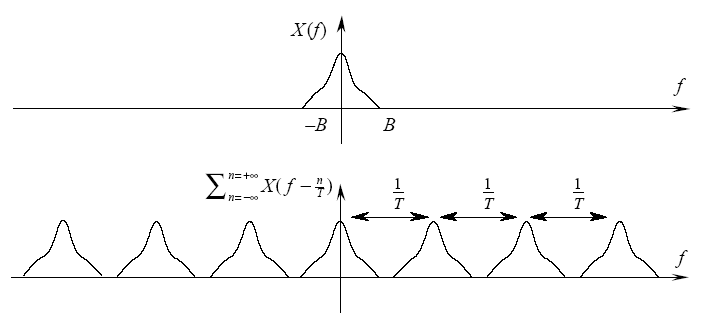
\includegraphics[width=12cm]{img/cons_ech_01}
    \caption{Lien entre la fr�quence d'�chantillonnage d'un signal et la p�riodisation de son spectre.}
    \label{sch_ech}
\end{figure}


Il peut survenir un probl�me si la fr�quence d'�chantillonnage $F_e$ est trop petite car les ��r�pliques�� p�riodiques du spectre  peuvent se superposer partiellement comme le montre la figure \ref{sch_repli}.

\vspace{5mm}

\begin{figure}[h]
     \centering
     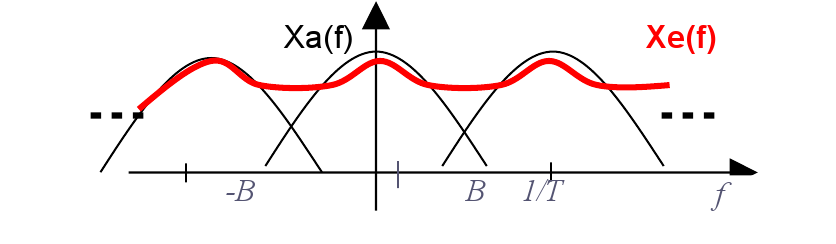
\includegraphics[width=12cm]{img/repliement}
     \caption{Ph�nom�ne de repliement.}
     \label{sch_repli}
\end{figure}


Cela arrive si la borne sup�rieure d'un �l�ment de $X_a(f)$ est plus grande que la borne inf�rieure de l'�lement suivant, autrement dit si $B < \frac{1}{T} - B$ o� $B$ est la fr�quence maximale contenue dans le signal (cf. fig. \ref{sch_repli}).

Ainsi, pour que le spectre $X_a(f$) ne soit pas ��d�form頻 lors de sa p�riodisation, il faut donc que�:

\begin{equation}\label{shannon}
 \boxeq{Fe > 2 B}
\end{equation}

Cette condition constitue le \textbf{th�or�me de Shannon} �nonc� ainsi : <<~la fr�quence d'�chantillonnage d'un signal doit �tre �gale ou sup�rieure au double de la fr�quence maximale contenue dans ce signal~>>.


\section{La transform�e en Z}

\subsection{D�finition de la transform�e en Z}

Pour d�crire un filtre dans le domaine num�rique, il est pratique de d�finir une transform�e dont la variable a la m�me nature que celle du signal discr�tis�. En effet, un signal num�rique - discontinu de nature - ne comporte qu'un nombre fini de valeurs et on a besoin d'une transform�e � temps discret pour d�crire les filtres : la transform�e en $Z$.

Soit $x(n)$ un signal discret quelconque. Sa transform�e en Z s'�crit :

\begin{equation}
X(z) = \mathcal{Z}\{x(n)\} =\sum_{n=-\infty}^{+\infty}x(n)z^{-n},\quad z \in \{z\in\mathbb{C}|\sum_{n=-\infty}^{+\infty}x(n)z^{-n} \quad converge\}
\end{equation}

Remarque : on retrouve la d�finition de la transform�e de Fourier en posant $z = e^{j2\pi f}$.

\subsection{Existence de la transform�e en Z}

Le domaine de convergence est le sous-ensemble de $\mathbb{C}$ dans lequel la s�rie converge.
Autrement dit, le domaine de convergence de la transform�e en z de la suite ($x_{n})_{n\in\mathbb{Z}}$ est l'ensemble :
	
\begin{equation}
\left\{z\in\mathbb{C} | \sum_{n=-\infty}^{\infty}x_{n}z^{-n} \quad\mathrm{existe}\right \}
\end{equation}

On l'appelle �galement couronne de convergence. En effet, en posant $z=\rho e^{i\theta}~$, il vient :

\begin{equation}
|X(z)|=\left| \sum_{n=-\infty}^{\infty}x_{n}z^{-n}\right|\leq \sum_{n=-\infty}^{\infty}\left|x_{n}\right|\rho^{-n}
\end{equation}

Donc $X(z)$ existe si $x(n)$ a une croissance au plus exponentielle, auquel cas le domaine de convergence est compris dans une couronne :

\begin{itemize}
\item de petit rayon le majorant de la base du c�t� des n n�gatifs
\item de grand rayon le majorant de la base du c�t� des n positifs
\end{itemize}

Dans toute la suite de l'article, les transform�es en Z ne seront valables que dans ce domaine de convergence sans que cela soit repr�cis�.

\subsection{Propri�t�s de la transform�e en Z}

\begin{enumerate}
\item\textbf{ Lin�arit�}
La transform�e en Z d'une combinaison lin�aire de deux signaux est la combinaison lin�aire des transform�es en Z de chaque signal.

\begin{equation}
  \mathcal{Z}\{a_1 x_1(n) + a_2 x_2(n)\} = a_1 \mathcal{Z}\{x_1(n)\} + a_2 \mathcal{Z}\{x_2(n)\}
\end{equation}

\item \textbf{D�calage temporel}

Le d�calage temporel d'un signal de k �chantillons se traduit par la multiplication de la transform�e en Z du signal par $z^k$.

\begin{equation}
\mathcal{Z}\{x(n-k)\} = z^{-k}\mathcal{Z}\{x(n)\}
\end{equation}

\item \textbf{Convolution}

La transform�e en Z d'un produit de convolution est le produit des transform�es en Z

\begin{equation}
\mathcal{Z}\{x(n) \star y(n)\} = \mathcal{Z}\{x(n)\} \mathcal{Z}\{y(n)\} \                                                                      \end{equation}

\item \textbf{Multiplication par une exponentielle}

\begin{equation}
\mathcal{Z}\{a^{n}x(n)\} = X\left(\frac{z}{a}\right)
\end{equation}

\item \textbf{Multiplication par la variable d'�volution}

De fa�on g�n�rale :

\begin{equation}
\mathcal{Z}\{n^{k}x(n)\} = \left(-z \frac{\mathrm{d} }{\mathrm{d}z}\right)^{k}\mathcal{Z}\{x(n)\}\                                               \end{equation}

o� $\textstyle\left(-z \frac{\mathrm{d} }{\mathrm{d}z}\right)^{k}\mathcal{Z}\{x(n)\}$ signifie que l'on applique $k$ fois � $\mathcal{Z}\{x(n)\} l'op�rateur \textstyle -z\frac{\mathrm{d} }{\mathrm{d}z}$

Si l'on �crit cette formule au rang k=1, on obtient la formule de d�rivation :

\begin{equation}
\mathcal{Z}\{nx(n)\} = -z \frac{\mathrm{d} }{\mathrm{d}z}X(z)\
\end{equation}

\item \textbf{Th�or�me de la valeur initiale}

Soit $x(n)$\, un signal causal et $X(z)$\, sa transform�e en Z. Alors :

\begin{equation}
x(0) = \lim_{n \to 0}x(n)=\lim_{z \to +\infty}X(z)
\end{equation}

\item \textbf{Th�or�me de la valeur finale}

Soit $x(n)$, un signal causal et $X(z)$, sa transform�e en Z. Alors lorsque la limite existe, on peut �crire :

\begin{equation}
\lim_{n \to +\infty}x(n)=\lim_{z \to 1}(z-1)X(z)
\end{equation}

\end{enumerate}


\chapter{Syst�mes lin�aires et filtrage}
\section{Introduction}

Pour modifier l'�volution temporelle ou fr�quentielle d'un signal d�termin�, on a g�n�ralement recours � des \textit{fonctions} temporelles ou fr�quentielles qui s'appliquent aux valeurs du signal. Ces fonctions peuvent �tre regroup�es au sein d'un syst�me filtrant $\mathbb{S}$ nomm� \textit{filtre} d�livrant un signal $y(t)$ en r�ponse � une stimulation  $x(t)$. On peut donc �crire, si $S$ est la fonction du filtre :

\begin{equation}
 y(t)=S[x(t)]
\end{equation}

D'un point de vue tr�s g�n�ral, on peut consid�rer que tout signal transitant dans une cha�ne de transmission est soumis � une op�ration de filtrage. Voici quelques exemples de filtres :

\begin{itemize}
 \item un syst�me de mesure con�u pour d�tecter la pr�sence d'un signal de forme particuli�re,
 \item un filtre �lectronique, un amplificateur, un convertisseur A/D,
 \item un algorithme informatique agissant sur un signal num�rique.
\end{itemize}

Le pr�sent chapitre constitue une synth�se de la th�orie des filtres analogiques et num�riques qui tente de donner les �l�ments de description des transformations temporelles ou fr�quentielles - comme par exemple la r�ponse impulsionnelle - qu'op�re $\mathbb{S}$ sur les signaux r�els. L'objectif est �galement de comprendre les m�thode de conception de la fonction de filtrage $S$ pour r�aliser une op�ration particuli�re. Enfin, il sera donn� quelques m�thodes pour d�terminer les propri�t�s de la fonction $S$ en observant les r�ponses du syst�me � des simulations ext�rieures.


\section{R�ponse impulsionnelle d'un syst�me}

Il est possible de d�crire un syst�me $\mathbb{S}$ par l'interm�diaire de sa r�ponse � des signaux particulier. Math�matiquement, une m�thode efficace est de d�terminer la r�ponse de $\mathbb{S}$ � une impulsion de Dirac, \cad une la \textbf{r�ponse impulsionnelle} telle que :

\begin{equation}
 s_{\delta}(t) = S(\delta(t))
\end{equation}

Le signal $s_{\delta}(t)$ r�cup�r� constitue une signature caract�ristique du filtre. En effet, la transform�e de Fourier d'une impulsion �tant une constante (dans le l'espace des fr�quences) la transform�e de Fourier de la r�ponse impusionnelle donne la r�ponse fr�quentielle du filtre pour toutes les fr�quences. Ainsi, il est possible de mesurer rapidement le comportement de n'importe quel filtre. La r�ponse d'une salle acoustique, par exemple, peut �tre �valu�e avec un explosif ou un autre son bref.

Dans la nature, tous les signaux sont \textbf{causaux}, \cad que les �l�ments du signal $y(t)$ ne peuvent exister avant ceux de $x(y)$. En d'autres termes, la causalit� impose qu'un signal ne peut pr�c�der celui qui lui a donner naissance\footnote{En math�matique, il est possible de d�finir des filtres non-causaux, mais cela n'est pas l'objet ici.}. Ainsi les syst�me causaux ont une r�ponse impulsionnelle nulle avant l'instant d'impulsion, soit $y(t<0) = 0$. Par ailleurs, pour un syst�me causal, le signal de sortie � l'instant $t$ d�pend du signal d'entr�e aux instants $t'< t$. La dur�e de la r�ponse impulsionnelle $s_{\delta}(t)$ correspond au temps de r�ponse du syst�me.

Une fois la r�ponse impulsionnelle connue, on peut pr�dire la r�ponse du filtre $y(t)$ issue de n'importe quel signal d'entr�e $x(t)$ gr�ce au produit de convolution�:

\begin{equation}
y(t) = x(t) \star s_{\delta}(t)
\end{equation}


\section{R�ponse fr�quentielle d'un syst�me}

La r�ponse en fr�quence d'un syst�me correspond � la transform�e de Fourier de la r�ponse impulsionnelle du syst�me.

$G(f)$ d�crit comment la distribution spectrale d'un signal est modifi�e ou "filtr�e" par le syst�me $\mathbb{S}$. Il est important de noter que le syst�me peut seulement modifier des composantes spectrales mais ne peut en aucun cas en cr�er de nouvelles. $\vert G(f) \vert$  est le gain du syst�me, c'est � dire la fa�on dont il modifie les amplitudes de chaque composantes spectrales. $Arg[G(f)]$ repr�sente le d�phasage caus� par le syst�me, c'est � dire le <<�retard�>> ou l'<< avance >> qu'il impose � certaines composantes spectrales.

La r�ponse en fr�quence, comme la r�ponse impulsionnelle permet de d�crire compl�tement le syst�me et de pr�dire la r�ponse du syst�me � n'importe quelle entr�e. Nous retrouvons l'�quivalence entre le produit de convolution dans le domaine temporel et le produit scalire dans le domaine fr�quentiel :

\begin{equation}
y(t) = x(t) \star g(t) \Leftrightarrow Y(f)  = X(f) . G(f)
\end{equation}

Ainsi, la fonction de transfert $G(f)$ d'un syst�me constitue le rapport entre signal re�u et le signal �mis dans le domaine fr�quentiel tel que :

\begin{equation}
 G(f) = \frac{Y(f)}{X(f)}
\end{equation}


\section{Filtrage}

Le filtrage lin�aire est une op�ration utile pour s�lectionner une partie du spectre d'un signal ou en att�nuer une partie, pour
modifier le contenu spectral d'un signal  ou encore mod�liser la transformation d'un signal dans un conduit propagatif, dans une salle.

Pour tous les filtres, on peut d�terminer une fonction de transfert �gale au rapport entre spectre du signal de sortie et celui du signal d'entr�e :

\begin{equation}
 G(f) = \frac{Y(f)}{X(f)}
\end{equation}

Cette fonction de transfert peut aussi s'�crire dans l'<< espace Z >> :

\begin{equation}
 G(z) = \frac{Y(z)}{X(z)}
\end{equation}

Ainsi la connaissance de la fonction de transfert d'un filtre nous renseigne compl�tement sur sa nature, quelque soit l'espace de repr�sentation. La fonction de transfert d'un filtre num�rique est donc d�finie comme la transform�e en $Z$ de la r�ponse impulsionnelle du filtre.

Nous n'aborderons pas dans ce cours la description de la transform�e de Laplace\footnote{\url{http://fr.wikipedia.org/wiki/Transform�e_de_Laplace}} qui est le pendant de la transform�e en Z dans le domaine analogique, c'est-�-dire temps continu. Mais il est essentiel de bien la conna�tre pour concevoir des filtres analogiques.

\subsection{Filtres classiques - vocabulaire}

On d�finit ici 4 types de filtres les plus classiques�:

\begin{itemize}
\item les filtres \textbf{passe-bas} qui laissent intact les basses fr�quences d'un signal et en att�nuent les hautes fr�quences,
\item les filtres \textbf{passe-haut} qui laissent intact les hautes fr�quences d'un signal et en att�nuent les basses fr�quences,
\item les filtres \textbf{passe-bande} qui s�lectionnent une partie du spectre d'un signal autour d'une fr�quence sp�cifi�e, avec une largeur plus ou moins grande,
\item les filtres \textbf{coupe-bande}, qui att�nuent fortement une partie du spectre d'un signal autour d'une fr�quence sp�cifi�e, avec une largeur plus ou moins grande.                                                                                                                     \end{itemize}


\begin{figure}[htp]
    \centering
    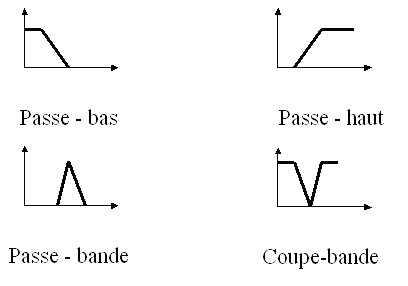
\includegraphics[width=8cm]{img/filtres_ideaux}
    \caption{Les filtres classiques. L'axe horizontal repr�sente la dimension fr�quentielle, l'axe vertical le module de la fonction de filtrage $|G(f)|$.}
    \label{filtres_ideaux}
\end{figure}

Pour tous ces filtres, on d�finit des \textbf{fr�quences de coupure}, c'est � dire les fr�quences pour lesquelles le spectre du signal d'entr�e va �tre att�nu� d'un facteur $\sqrt{2}$ par rapport � la valeur maximale du spectre d'amplitude. Cette variation �quivaut � une variation de 3 dB dans l'�chelle logarithmique.

Le filtre  passe-bas � donc une fr�quence de coupure dans les m�diums / hautes fr�quences, le passe haut une fr�quence de coupure dans les m�diums / basses fr�quences. Les passe bande et coupe bande poss�dent deux fr�quences de coupure autour de la fr�quence centrale sur laquelle ils se centrent. On sp�cifie �galement la pente de l'att�nuation de ces filtres, en dB par octave qui apporte une information sur la \textbf{s�lectivit�} du filtre. Enfin, pour les filtres passe-bande et coupe-bande, on d�termine leur largeur de bande, c'est � dire la diff�rence entre leurs deux fr�quences de coupure qui renseigne aussi sur sa s�lectivit�.

\subsection{Filtres num�riques}

Avant de d�terminer sa fonction de transfert, un filtre num�rique peut-�tre d�fini par une �quation aux diff�rences, c'est-�-dire l'op�ration math�matique du filtre dans le domaine temporel discret entre le signal d'entr�e $x(n)$ quelconque et le signal filtr� de sortie $y(n)$. D'un point de vue g�n�ral, en respectant le principe de causalit�, tout signal filtr� $y(n)$ s'�crit comme un composition lin�aire des �chantillons pass�s de $x(n)$ et $y(n)$ tel que :

\begin{equation}
y(n) = {\sum_{k=0}^N} b_k  x(n-k) - {\sum_{k=1}^M} a_k y(n-k)\end{equation}

En calculant les transform�e en Z de chaque membre, on calcule ais�ment la fonction de transfert $H(z)$ dans le domaine z :

\begin{equation}
H(z) = \frac {Y(z)} {X(z)} = \frac {{\sum_{k=0}^N} b_k z^{-k}} {1 + {\sum_{k=1}^M} a_k z^{-k}}
\end{equation}

Les valeurs des coefficients $a_k$ et $b_k$ fixeront le type de filtre (passe-bas, passe-haut, et...).


\subsection{Exemples de filtres}

\subsubsection{Le filtre moyenneur lisseur}

Soit un signal num�rique $y(n)$ avec $n \in \mathbb{N}$ issu d'un signal $x(n)$ tel que :

\begin{equation}
 y(n)=\frac{x(n)+x(n-1)+x(n-2)+...+x(n-N+1)}{N}
\end{equation}

La transform�e en $Z$ de $y(n)$ s'�crit alors :

\begin{eqnarray}
 Y(z) & = & \sum_{p=0}^{N-1} X(z)\frac{z^{-p}}{N} \\
      & = & X(z) \sum_{p=0}^{N-1}\frac{z^{-p}}{N}
\end{eqnarray}

On en d�duit la fonction de transfert $H(z)$ du filtre �quivalent :

\begin{equation}
 H(z)=\frac{Y(z)}{X(z)} = \sum_{p=0}^{N-1}\frac{z^{-p}}{N}
\end{equation}

\subsubsection{Le filtre passe-bas}

Soit $x(n)$ un signal num�rique quelconque de fr�quence d'�chantillonnage $f_e$. La loi r�cursive qui produit un filtrage passe-bas de fr�quence de coupure $f_c$ pour obtenir le signal filtr� $y(n)$ s'�crit :

\begin{eqnarray}
 y(n) & = & y(n-1) + a [x(n)- y(n-1)] \\
 y(n) & = & a x(n)+[1-a] y(n-1) \\
 y(n) + [a-1] y(n-1) & = & a x(n) \label{filtre_pb}
\end{eqnarray}

en ayant pos� :

\begin{equation*}
 a = \frac{1}{1+\frac{f_e}{2 \pi f_c}}
\end{equation*}

En effectuant la transform�e de Z de chaque membre de l'�quation \ref{filtre_pb}, on obtient :

\begin{eqnarray}
  \sum_{n=-\infty}^{+\infty}y(n)z^{-n} + [a-1]  \sum_{n=-\infty}^{+\infty}y(n-1)z^{-n} & = & a \sum_{n=-\infty}^{+\infty}x(n)z^{-n} \\
  \sum_{n=-\infty}^{+\infty}y(n)z^{-n} + [a-1]  \sum_{n=-\infty}^{+\infty}y(n)z^{-n-1} & = & a \sum_{n=-\infty}^{+\infty}x(n)z^{-n} \\
  Y(z) + [a-1]  Y(z) . z^{-1} & = & a X(z) \\
  \frac{Y(z)}{X(z)} = \frac{a}{1+(a-1)z^{-1}}
\end{eqnarray}

D'un point de vue pratique, c'est cette fonction qui permet d'impl�menter - c'est � dire de mettre en oeuvre sous la forme d'un programme - la fonction de filtrage de type passe-bas dans un programme informatique. Dans le logiciel libre Octave\footnote{\url{http://www.octave.org}}, le code suivant permet par exemple de tester ce filtrage sur des signaux al�atoires � partir de la loi r�cursive mais aussi en utilisant la fonction \verb|filter| :

\begin{verbatim}
% Script Matlab / Octave pour tester une fonction de filtrage passe-bas.

f0 = 20;
f1 = 22050;
t1 = 1;
fe = 44100;
fc = 3000;
a = 1/(1+fe/(2*pi*fc));

t = [0:1/fe:t1];
n = length(t);
N = 10;

for k=1:N

    s = randn(1,n);
    %sweep = sin(2*pi*(f0*t1)/log(f1/f0) * (exp(t'/t1*log(f1/f0))-1))';
    sf(1) = s(1);

    % Avec une boucle
    tic;
    for i=2:n
        sf(i)=a*s(i)+(1-a)*sf(i-1);
    end
    t_boucle(k) = toc;

    % Avec filter
    tic;
    sff = filter(a,[1 a-1],s);
    t_filter(k) = toc;

    % Fonction de transfert
    nfft = 16384;
    fft_s = fft(s,nfft);
    fft_sf = fft(sf,nfft);
    fft_sff = fft(sff,nfft);
    f = [0:fe/nfft:fe/2];
    f(1) = [];

    mod_FT(k,:) = abs(fft_sf)./abs(fft_s);
    pha_FT(k,:) = angle(fft_sf);
    mod_FTF(k,:) = abs(fft_sff)./abs(fft_s);
    pha_FTF(k,:) = angle(fft_sff);

end

mod_FT = mean(mod_FT);
figure(1)
semilogx(f,20*log10(mod_FT(1:nfft/2)));
hold on
semilogx(f,20*log10(abs(1./(1+j*(f/fc)))),'r');
title(['Module de la fonction de transfert par la methode recursive (reel / theorique)']);
xlabel(['Frequence (Hz)']);
ylabel(['Amplitude (dB)']);

pha_FT = mean(pha_FT);
figure(2)
semilogx(f,unwrap(pha_FT(1:nfft/2)));
xlabel(['Frequence (Hz)']);
ylabel(['Phase (rad)']);
title(['Phase de la fonction de transfert par la m�thode recursive']);

mod_FTF = mean(mod_FTF);
figure(3)
semilogx(f,20*log10(mod_FTF(1:nfft/2)));
hold on
semilogx(f,20*log10(abs(1./(1+j*(f/fc)))),'r');
title(['Module de la fonction de transfert par la fonction filter (reel / theorique)']);
xlabel(['Frequence (Hz)']);
ylabel(['Amplitude (dB)']);

pha_FTF = mean(pha_FTF);
figure(4)
semilogx(f,unwrap(pha_FTF(1:nfft/2)));
xlabel(['Frequence (Hz)']);
ylabel(['Phase (rad)']);
title(['Phase de la fonction de transfert par la fonction filter']);

figure(5)
plot(t_boucle);
title(['Temps d execution (s)']);
hold on
plot(t_filter,'r');

pause;

\end{verbatim}

Pour plus d'exemple sur les fonctions num�rique de filtrage, voir \url{http://math.fullerton.edu/mathews/c2003/ZTransformFilterMod.html}.

\subsubsection{Le filtre vocal}

On peut mod�liser la sensation d'intensit� auditive par un filtre. L'oreille humaine est particuli�rement sensible entre 3 et 4 kHz.

\begin{figure}[htp]
    \centering
    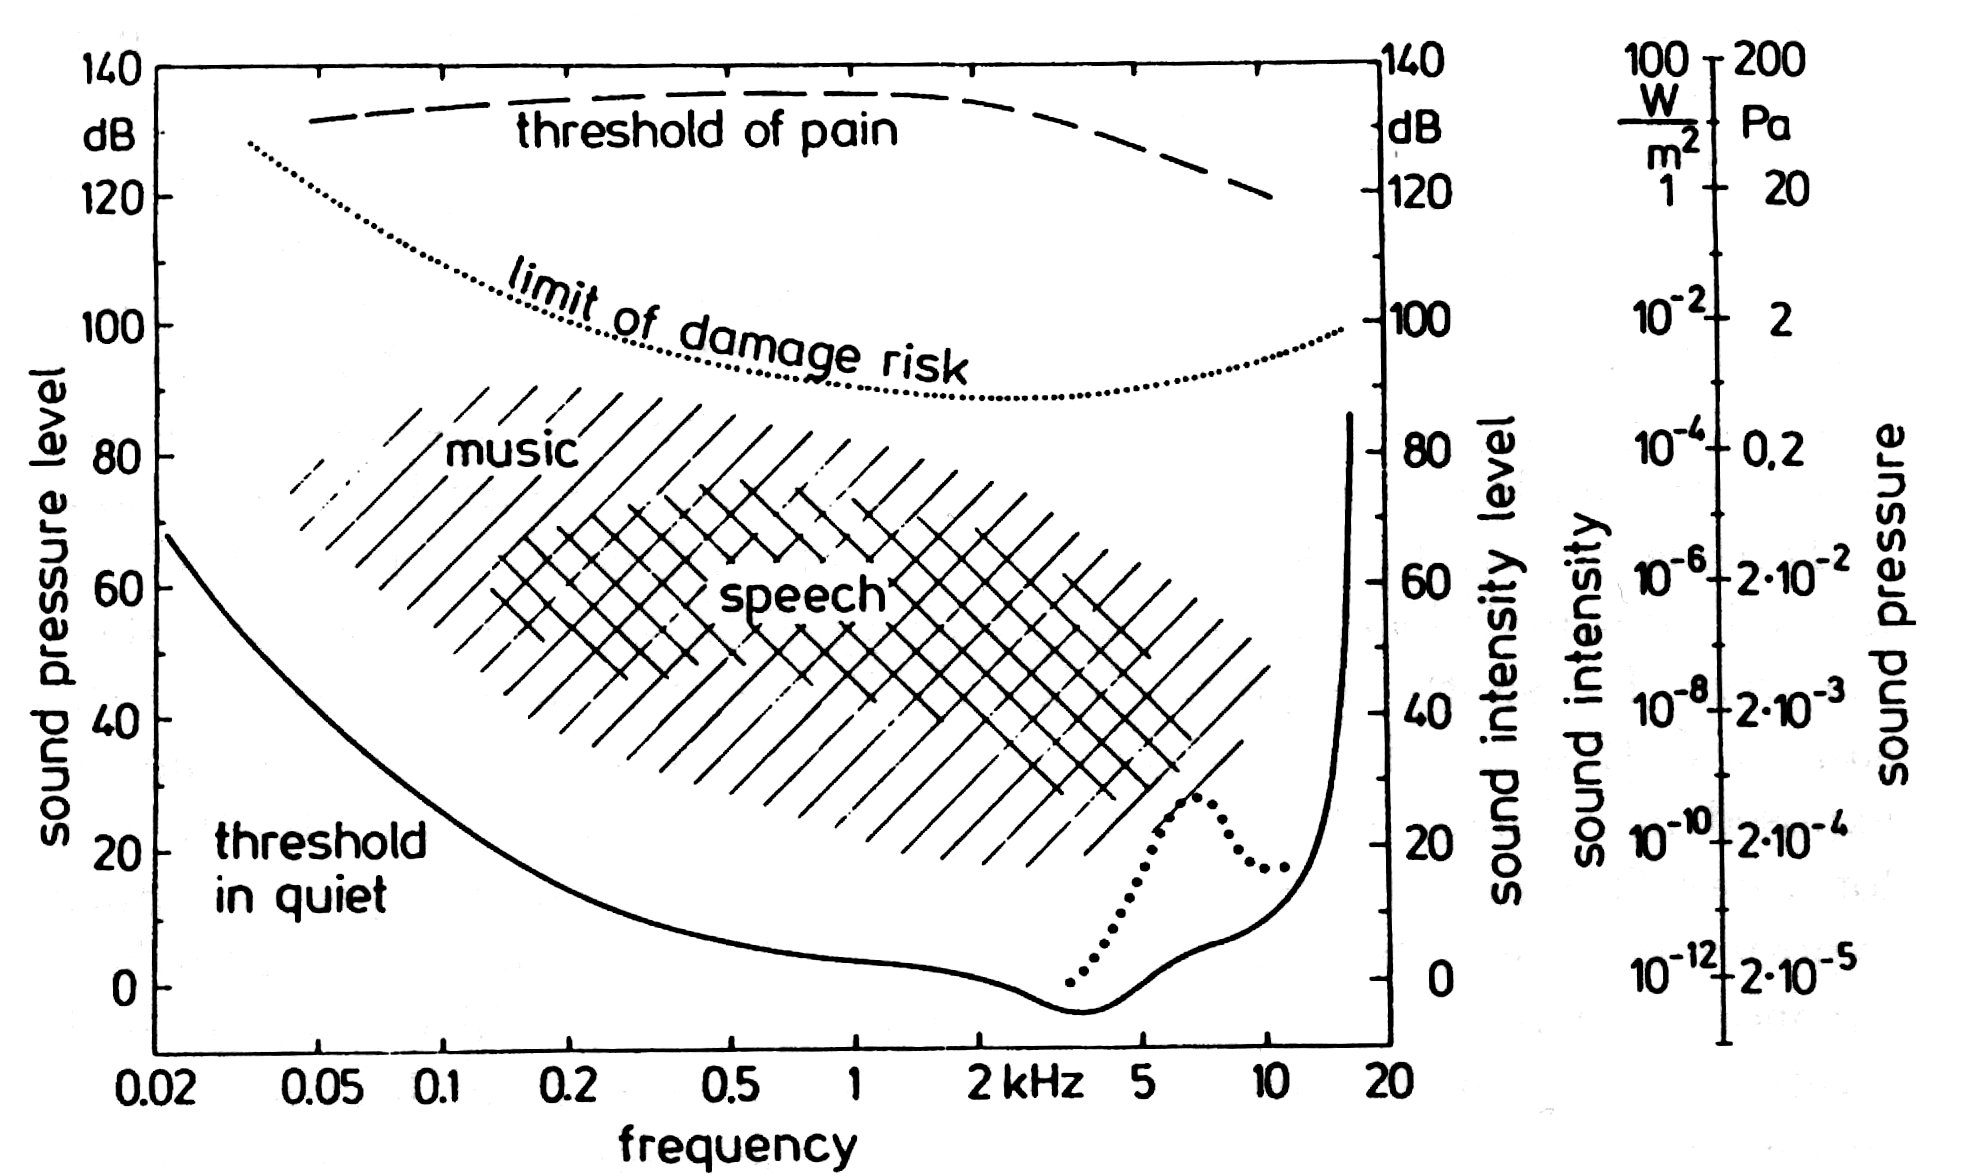
\includegraphics[width=12cm]{img/sens_oreille}
    \caption{Diagramme de sensibilit� de l'oreille humaine.}
    \label{sens_oreille}
\end{figure}

On peut �galement mod�liser la production phonatoire par un mod�le source-filtre, o� le r�le de la source est jou� par les cordes vocales qui produisent un son harmonique avec une distribution de l'�nergie assez plate en fr�quence. Le conduit vocal, les fosses nasales ainsi que la place des articulateurs (langue, m�choire, l�vres) peuvent �tre mod�lis�s par un filtre qui modifie le son glottique pour produire le son tel que nous le percevons � la sortie des l�vres d'un locuteur.

\begin{figure}[htp]
    \centering
    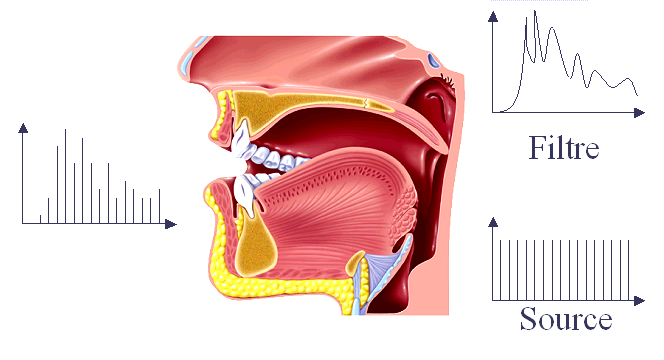
\includegraphics[width=12cm]{img/sf_voix}
    \caption{Mod�le source/filtre de la voix.}
    \label{sf_voix}
\end{figure}



\chapter{Modes de repr�sentation des signaux}
\section{Fen�trage des signaux}

Nous avons vu dans le chapitre pr�c�dent que la Transform�e de Fourier permet de repr�senter le spectre d'un signal dans le domaine fr�quentiel. Pour une sinuso�de infinie, toute l'�nergie du spectre est concentr�e � une fr�quence donn�e, c'est � dire la fr�quence de la sinuso�de (cf. fig. \ref{ft_sin}).

\begin{figure}[htbp]
    \centering
    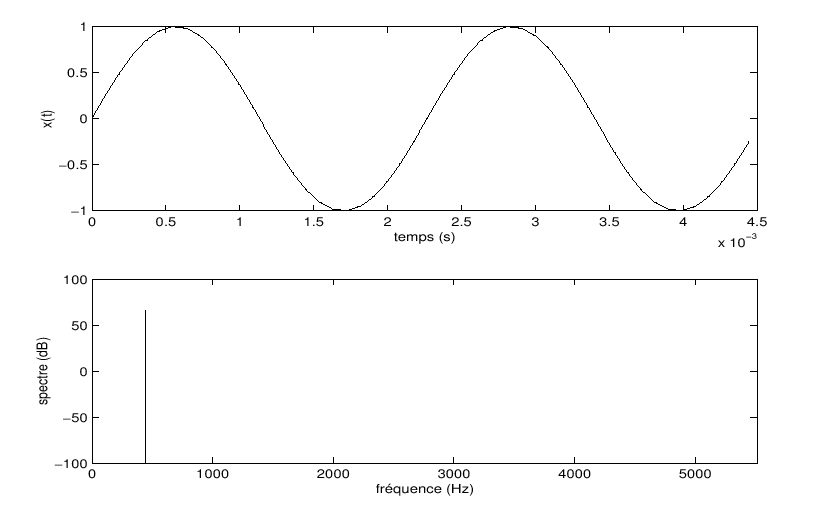
\includegraphics[width=12cm]{img/ft_sin}
    \caption{Repr�sentation temporelle et spectre d'une sinuso�de dit << son pur >>.}
    \label{ft_sin}
\end{figure}

Si on veut observer ce sinus sur un temps fini, on va �tre oblig� de le tronquer. L'�nergie va alors d'une part se r�partir autour de la fr�quence de la sinuso�de. C'est ce qu'on appelle l'\textbf{�talement spectral}. D'autre part, on observe la pr�sence d'�nergie dans toutes les fr�quences. Ce ph�nom�ne est appel� \textbf{fuite spectrale} (cf. fig. \ref{ft_sin_01}). L'�talement et fuite sont directement li�s � la troncature.

\begin{figure}[htp]
    \centering
    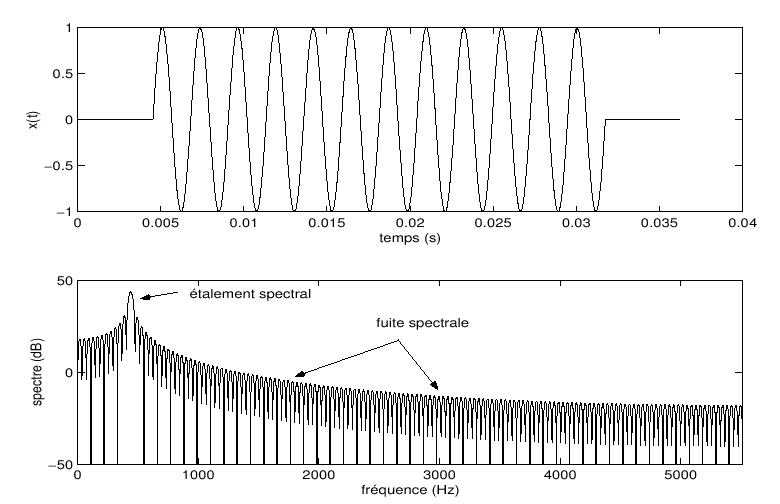
\includegraphics[width=12cm]{img/ft_sin_01}
    \caption{Repr�sentation temporelle et spectre d'une sinuso�de tronqu�e.}
    \label{ft_sin_01}
\end{figure}

\begin{figure}[htp]
    \centering
    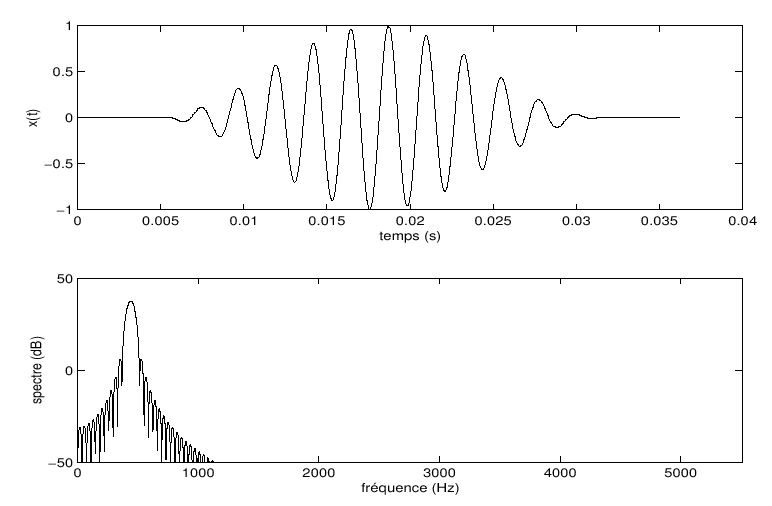
\includegraphics[width=12cm]{img/ft_sin_fen}
    \caption{Repr�sentation temporelle et spectre d'une sinuso�de modul�e par une fen�tre de Hanning.}
    \label{ft_sin_fen}
\end{figure}

Si on r�alise la troncature de fa�on non rectangulaire mais en ��fen�trant�� le signal - par une fen�tre de Hanning par exemple, (cf.  fig. \ref{ft_sin_fen}) - les transitions dans le signal sont alors plus douces. La fuite spectrale est alors limit�e mais l'�talement en fr�quence est toujours pr�sent. Ce point est important pour comprendre le r�le des \textbf{fen�tres d'analyse}. Si la fen�tre a des discontinuit�s fortes, les fuites spectrales vont �tre importantes, mais l'�talement moindre. Si on prend une fen�tre de discontinuit� plus douce, on va au contraire obtenir un �talement plus grand, mais moins de fuites spectrales.


\section{Le spectrogramme}

L'int�r�t du spectrogramme est de pouvoir repr�senter le spectre en �voluant dans le temps. Le nom scientifique de la fonction math�matique associ�e � cet outil, plus commun�ment appel� ��spectrogramme��, est la Transform�e de Fourier � Court Terme (TFCT). Ce nom provient de l'analyse effectu�e sur des fen�tres de support temporel fini. Une autre d�nomination de cette repr�sentation est ��sonagramme��. Il s'agit d'une marque d�pos�e Kay Electronics.

Le principe du spectrogramme est de ��d�couper�� le son en trames. Pour chacune de ces trames on calcule une transform�e de Fourier comme le sch�matise la figure \ref{tfct}. Ce spectre est alors repr�sent� � un temps correspondant � celui du centre de la fen�tre, sous forme d'un code de couleur.

\begin{figure}[htbp]
    \centering
    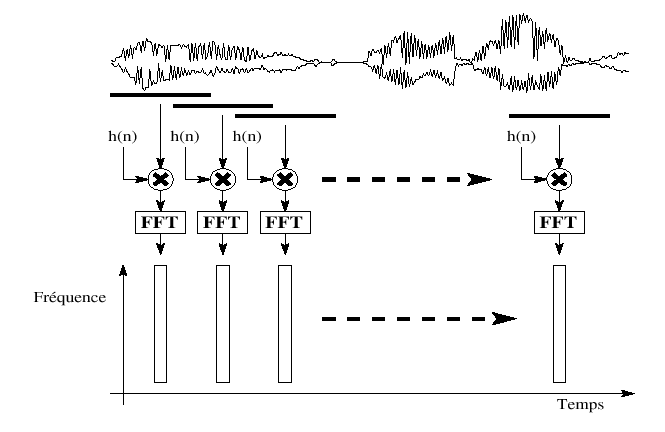
\includegraphics[width=12cm]{img/tfct}
    \caption{Description sch�matique de l'analyse temps/fr�quence par la FFT.}
    \label{tfct}
\end{figure}

La figure \ref{spectr_voix1} montre un exemple de spectrogramme d'un �chantillon sonore de voix chant�e. Il s'agit d'un glissando C5-E5 r�alis� par une soprano. L'analyse a �t� effectu�e avec une fen�tre de Hanning de longueur 23 ms. Le jaune correspond aux amplitudes les plus fortes, le bleu/violet aux amplitudes les plus faibles. On a ainsi une id�e de l'aspect du spectre au temps t. A chaque calcul du spectre, le signal est fen�tr� de fa�on � pouvoir r�gler � la fois la fuite et l'�talement spectral. On observe facilement le glissando et le vibrato de la chanteuse.

\begin{figure}[htbp]
    \centering
    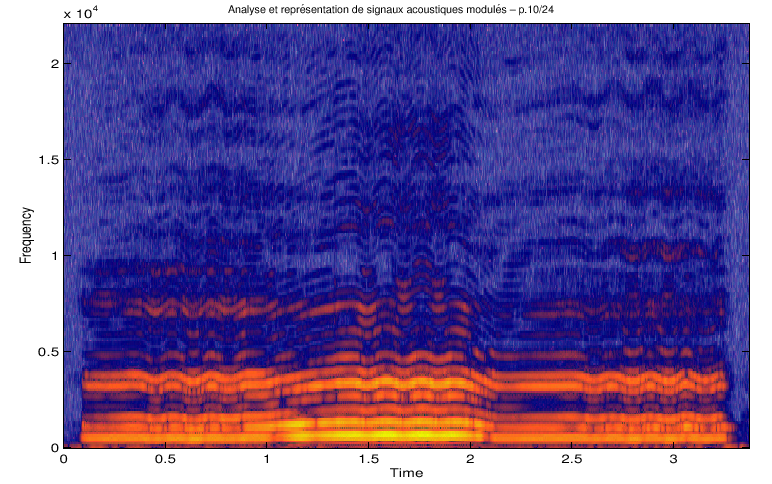
\includegraphics[width=12cm]{img/spectr_voix1}
    \caption{Spectrogramme d'un glissando C5-E5 r�alis� par une soprano (fen�tre : Hanning, 6 ms de largeur).}
    \label{spectr_voix1}
\end{figure}

Pour mesurer le vibrato par exemple, on serait tent� de r�duire la longueur de la fen�tre dans le temps pour gagner en pr�cision et suivre au mieux les variations du spectre. En r�alit�, si on r�duit la longueur des fen�tres (cf. fig. \ref{spectr_fen}), l'�talement spectral augmente, par cons�quent la largeur des raies sur le spectrogramme aussi, ce qui perturbe finalement la mesure, car on ne distingue plus distinctement les diff�rentes trajectoires dans le spectrogramme.

\begin{figure}[tp]
    \centering
    \subfigure[Fen�tre de 100 ms]{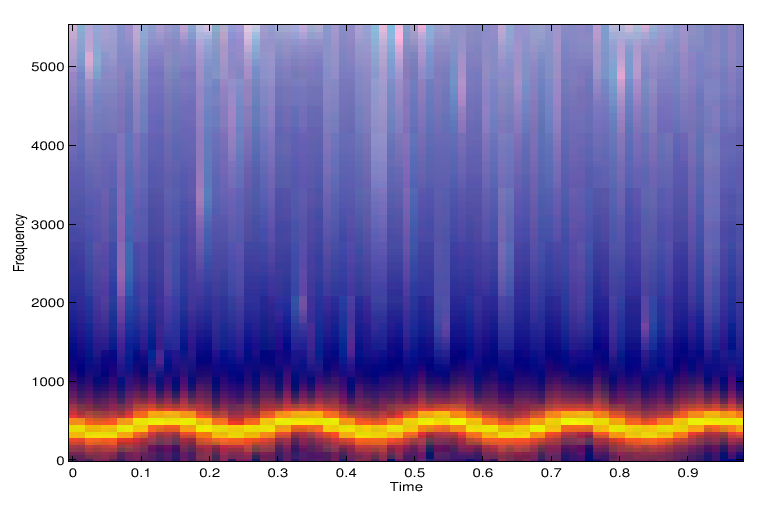
\includegraphics[width=8cm]{img/spectrogram_01.png}}
    \subfigure[Fen�tre de 20 ms]{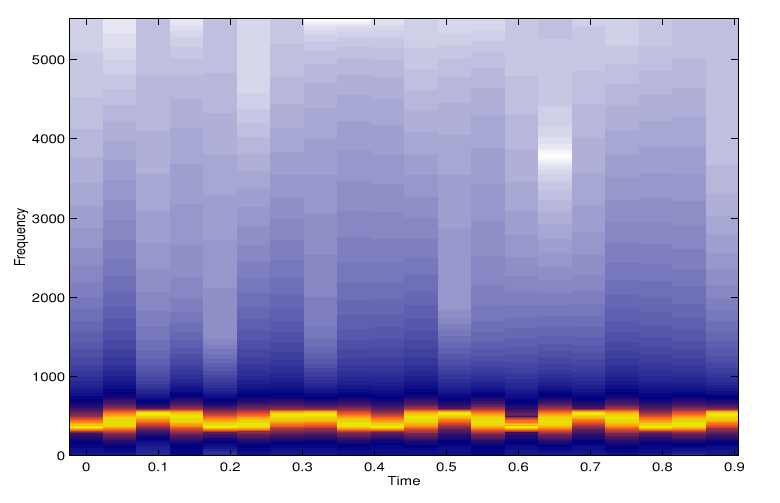
\includegraphics[width=8cm]{img/spectrogram_02.png}}
    \caption{Effet de la modification de la largeur d'une fen�tre temporelle lors du calcul d'un spectrogramme sur un signal contenant un vibrato.}
    \label{spectr_fen}
\end{figure}

Si on revient � la m�me longueur de fen�tre que dans le premier exemple, tout en utilisant une fen�tre rectangulaire au lieu de la fen�tre ��douce�� de Hanning, l'�talement spectral est plus faible et les lignes sur le spectrogramme plus fines. Dans ce cas, les fuites spectrales sont beaucoup plus importantes et caract�ris�es par un manque de contraste dans la repr�sentation du spectrogramme (cf. fig. \ref{spectr_fen_2}).

\begin{figure}[htbp]
    \centering
    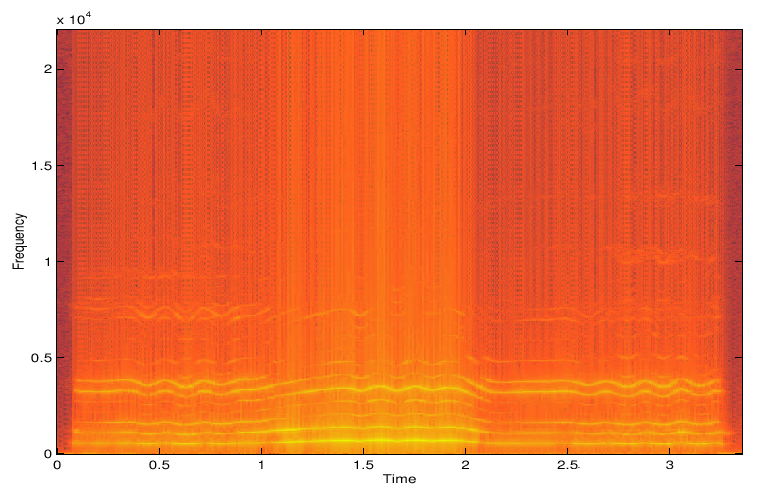
\includegraphics[width=12cm]{img/spectrogram_03.png}
    \caption{Spectrogramme d'un glissando C5-E5 r�alis� par une soprano (fen�tre : rectangulaire, 23 ms de largeur).}
    \label{spectr_fen_2}
\end{figure}

Les points importants quant � l'utilisation du spectrogramme�sont donc:
\begin{itemize}
 \item la longueur de fen�tre pour ajuster la pr�cision temporelle, au prix d'un �talement spectral qui peut devenir r�dhibitoire,
 \item le choix de la fen�tre qui va conditionner le contraste du spectrogramme, pour une longueur de fen�tre donn�e.
\end{itemize}


\section{Pertinence et choix d'un mode de repr�sentation}

La repr�sentation du signal en temporel est particuli�rement adapt� � l'analyse de ses variations temporelles, par exemple lors de l'attaque ou de l'extinction d'un son. Au contraire, cette repr�sentation apporte peu d'information lorsqu'on s'int�resse plut�t au contenu spectral du signal. Sur la figure \ref{spectr_voix2}, on voit que la repr�sentation spectrale de ces deux signaux de parole permet assez bien de diff�rentier la voix ��tendue��  de la voix ��rel�ch�e��.

\begin{figure}[tp]
    \centering
    \subfigure[Voix rel�ch�e]{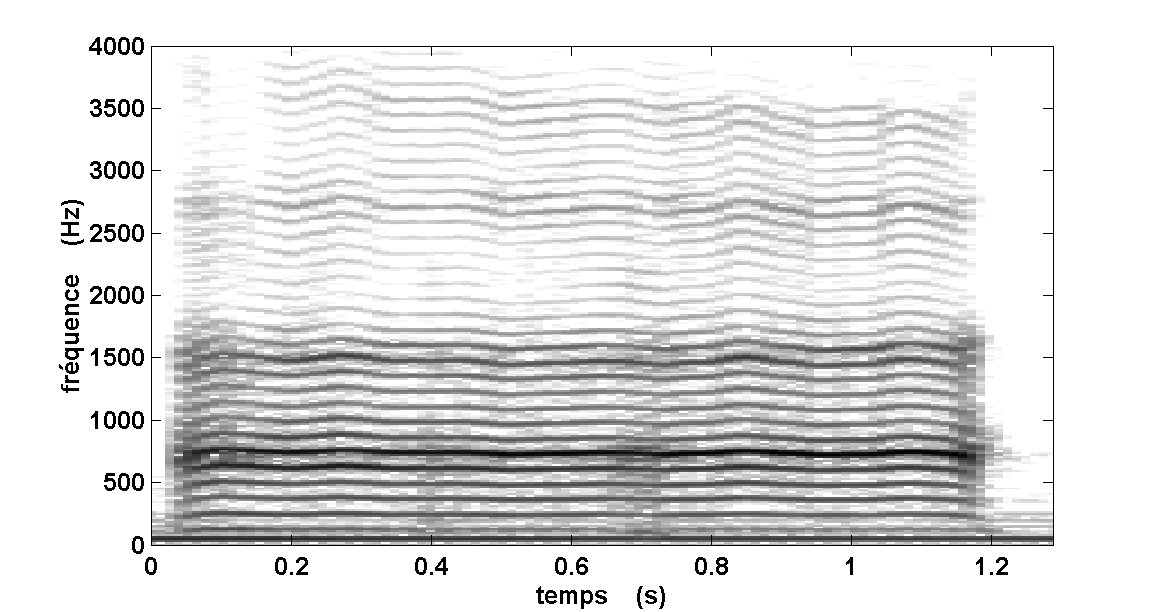
\includegraphics[width=8cm]{img/spectro_vibrato.png}}
    \subfigure[Voix tendue]{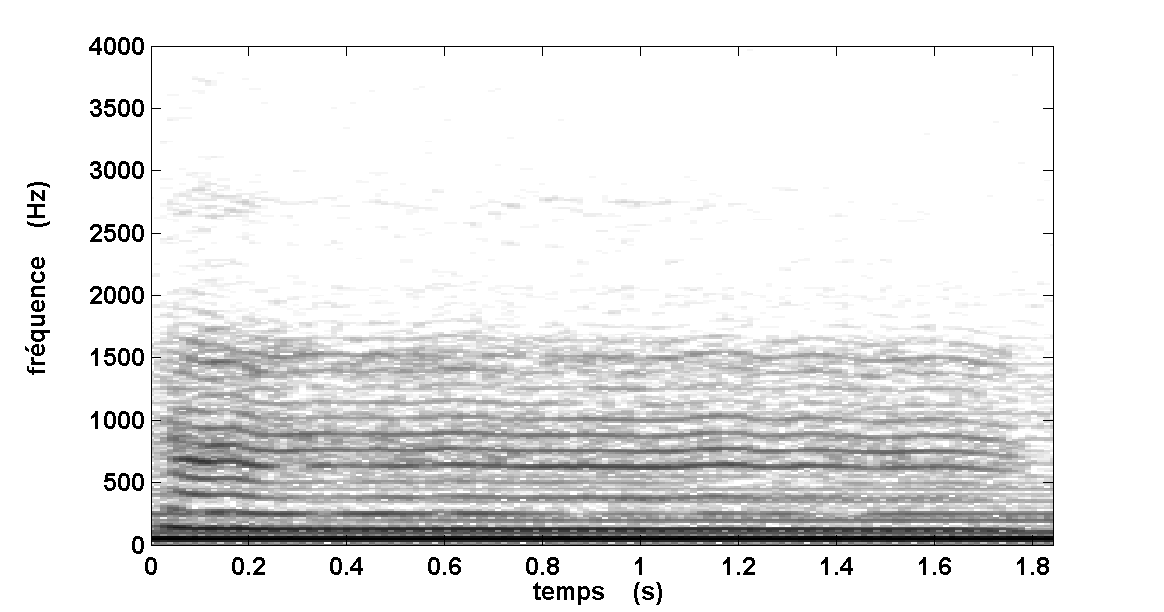
\includegraphics[width=8cm]{img/spectro_vibrato_2.png}}
    \caption{Spectrogrammes d'un son de voix rel�ch�e (A) et d'une voix tendue (B).}
    \label{spectr_voix2}
\end{figure}

Un autre int�r�t de la repr�sentation du signal � l'aide d'un spectrogramme est de pouvoir s�parer des sources sonores, \cad des structures, ou, tout du moins, de pouvoir rep�rer des �v�nements comme le montre la figure \ref{spectr_sep} o� l'on distingue deux structures spectrales distinctes.

\begin{figure}[htbp]
    \centering
    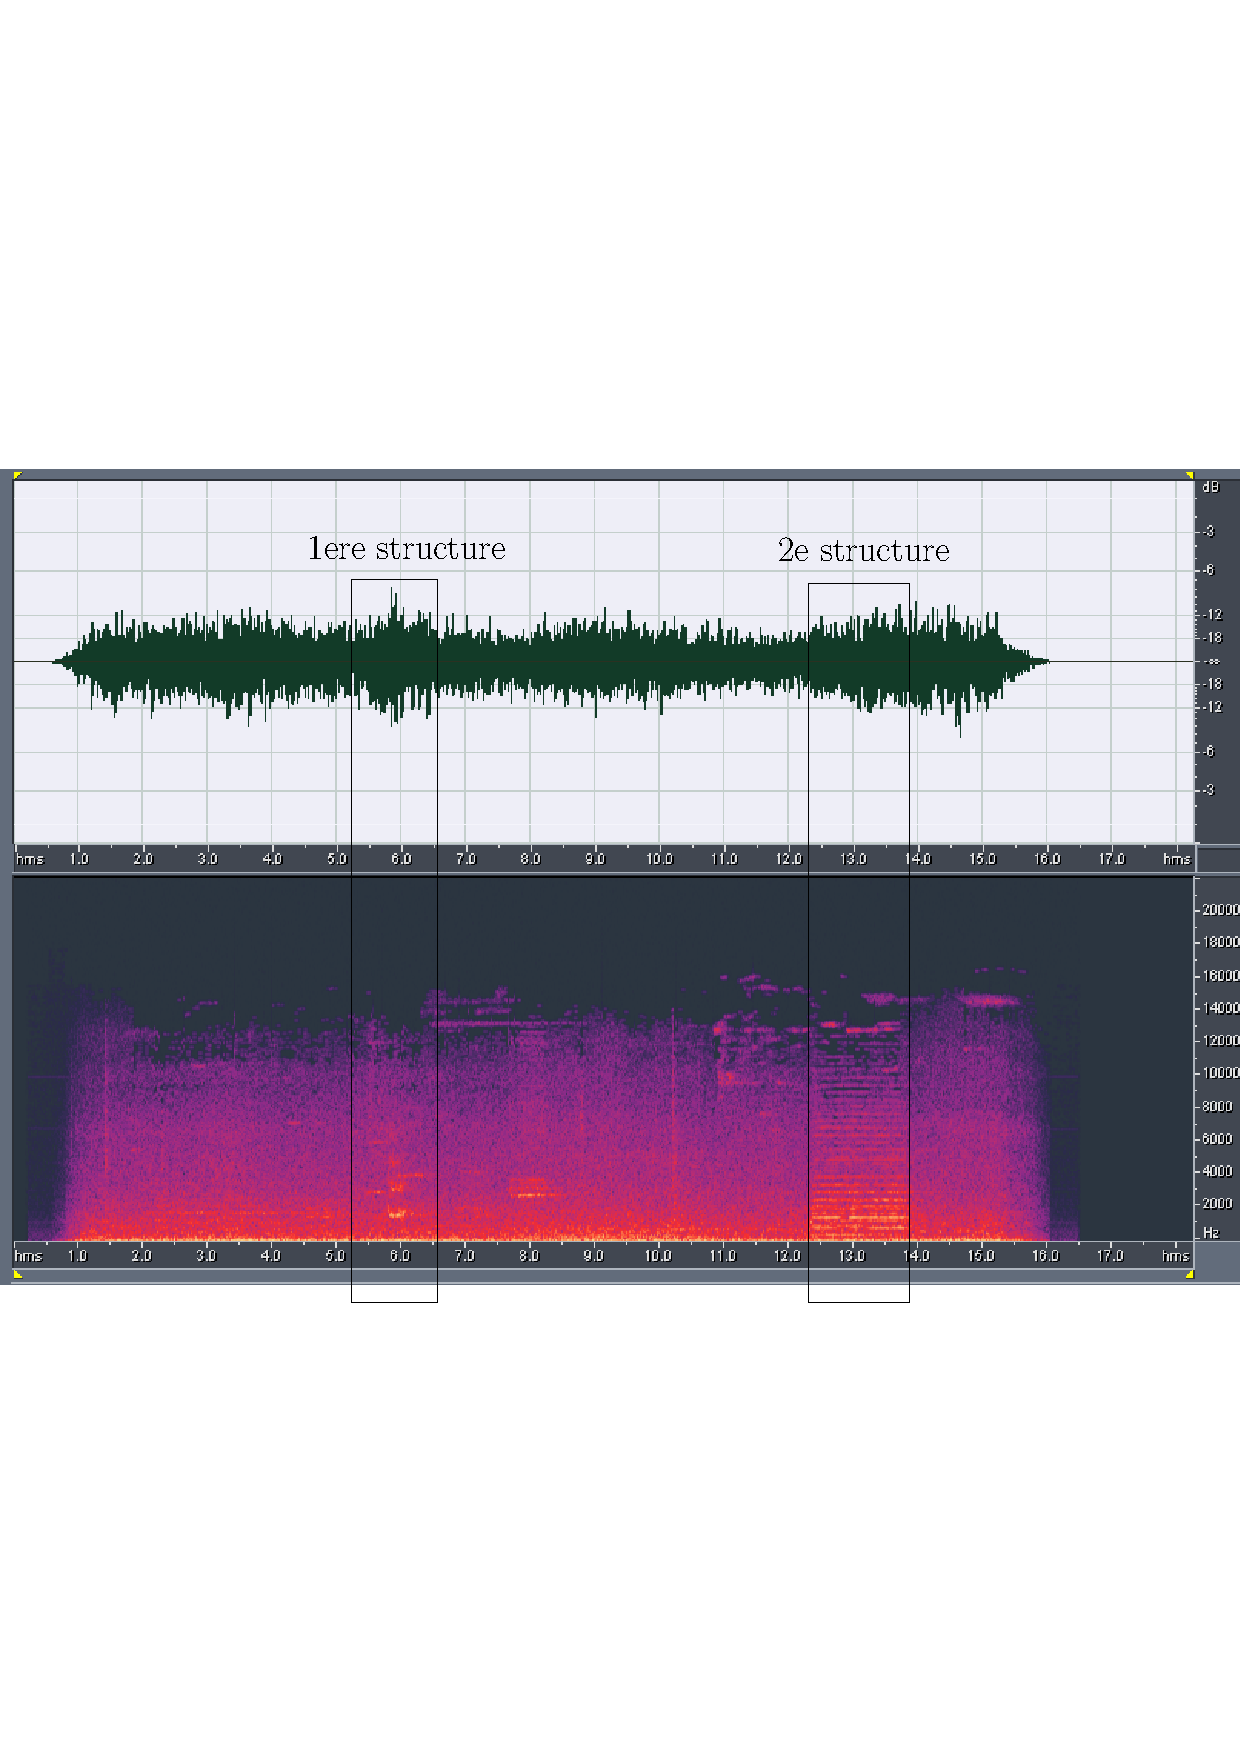
\includegraphics[width=12cm]{img/spectr_sep.pdf}
    \caption{Identification de structures sonores � l'aide d'un spectrogramme.}
    \label{spectr_sep}
\end{figure}


Pour des sons tr�s harmoniques, une voix chant�e par exemple, le spectrogramme permet de rep�rer tr�s facilement la fondamentale ainsi que la s�rie harmonique. La figure \ref{spectro_harm} repr�sente le spectrogramme d'un chanteur effectuant un glissando du bas au haut de sa tessiture puis l'inverse. On distingue facilement l'�volution temporelle de chaque harmonique contenu dans le signal.

\begin{figure}[htbp]
    \centering
    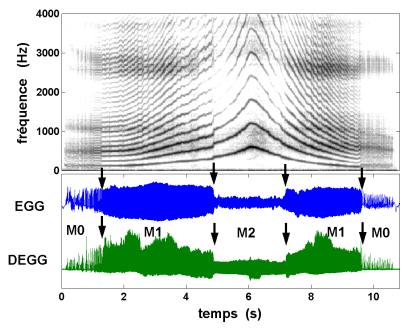
\includegraphics[width=12cm]{img/spectro_harm.png}
    \caption{Identification de l'�volution temporelle des harmoniques � l'aide d'un spectrogramme.}
    \label{spectro_harm}
\end{figure}

Dans le cas de la voix parl�e, on peut rep�rer les parties vois�e - harmoniques ou non - et m�me identifier quels sont les phon�mes prononc�s avec un peu d'exp�rience. Cette technique permet par exemple d'am�liorer les algorithme de reconnaissance vocale (cf. fig. \ref{spec_lux}).

\begin{figure}[htbp]
    \centering
    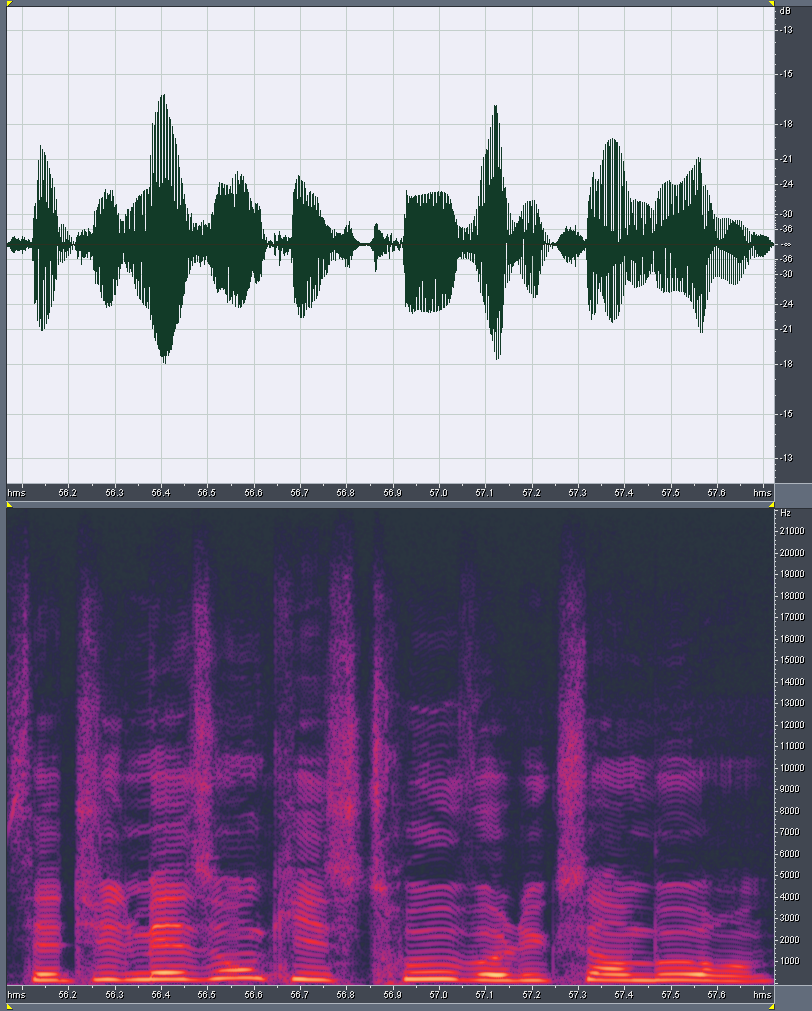
\includegraphics[width=12cm]{img/spec_lux.png}
    \caption{Identification de mots � l'aide d'un spectrogramme. Phrase : <<�C'est une maison qui s'trouve au Luxembourg�>>.}
    \label{spec_lux}
\end{figure}


\section{Le spectre moyenn� (Long Term Average Spectrum LTAS)}

Dans certains cas, il est �galement tr�s utile de repr�senter une partie du signal sous forme de spectre moyenn�. Le spectre moyenn� consiste � faire la moyenne du spectrogramme sur l'ensemble des instants d'un intervalle de temps. Cette op�ration peut �tre effectu�e sur le signal tout entier comme sur un morceau particulier.

Pour examiner une voyelle en particulier dans un signal de parole par exemple, il est tout � fait appropri� de moyenner le spectrogramme sur l'intervalle de temps de cette voyelle, de fa�on � pouvoir estimer les formants ou bien le contenu spectral de cette voyelle. Ainsi, sur la figure suivante, on peut examiner le spectre moyenn� de la production vocale d'un chanteur sur un /a/. Cette repr�sentation permet de caract�riser ses premiers formants vocaliques, ainsi que le formant du chanteur (renforcement �nerg�tique dans la zone 2000-4000 Hz) caract�ristique des chanteurs lyriques et des acteurs de th��tre.




\newpage
\bibliographystyle{plain}
\nocite{*}
\bibliography{bib/biblio}

\end{document}

